\documentclass{article}
\usepackage{booktabs}
\usepackage[labelfont=bf, format=hang]{caption}
\captionsetup[table]{position=bottom}

\usepackage{cite}
\usepackage{graphicx}
\usepackage{hyperref}
\usepackage[utf8]{inputenc}
\usepackage{multirow}
\usepackage{subfig}
\usepackage{tabularx}
\usepackage{url}


\title{%
    \textbf{Bioinformatics Course Project Report}\\
    \vspace{1em}
    Prediction of regulatory regions activity through deep learning methods
}
\author{%
    Gabriele Cerizza\\
    \url{gabriele.cerizza@studenti.unimi.it}\\
    \url{https://github.com/gabrielecerizza/bioinformatics_project}
}
\date{}

\begin{document}

\maketitle

\section{Introduction}

The regulation of gene expression is handled by non-coding regions that account for 98\% of the DNA. Chief among non-coding regions are those denoted as  “enhancers" and  “promoters". Promoters provide transcription factors binding sites to which, among other proteins, bind the RNA polymerase, which is the main enzyme responsible for gene transcription. Enhancers aid gene transcription by interacting with promoters. Enhancers can interact with promoters across hundreds of thousands of nucleotides \cite{kelley18}, by virtue of the peculiar three-dimensional folding structure of the DNA.   

Data-driven prediction of regulatory regions activity is crucial to understand the impact of genetic variations on phenotype, since variations that fall within inactive regulatory regions are less likely to be pathogenic \cite{cappelletti20}. In this endeavor, an important role is played by deep learning methods, owing to their capability to model complex non-linear functions starting from large quantities of data.

The application of deep learning methods in the context of regulatory regions has been an active field of research in recent years. Feed-Forward Neural Networks (FFNNs) trained on epigenomic data have been employed to distinguish promoters and enhancers, as well as active and inactive regulatory regions \cite{li_wasserman18, cappelletti20}. Convolutional Neural Networks (CNNs) trained on DNA sequences were used to identify promoters and distal regulatory elements \cite{min17, kelley18, cappelletti20, onimaru20, chen21} and to predict their activity \cite{cappelletti20}. Sometimes, CNNs have been trained also on epigenomic data \cite{chen21, chen_zhang21}.

Novel approaches combining data from different sources are being developed, exploiting several integration strategies. The joint consideration of heterogeneous information within the framework of Multi-Modal Neural Networks (MMNNs) shows improvements in the predictive power of deep learning models \cite{choi19, li_wu16}. 
In consideration of the foregoing, we hereby explore different deep learning architectures with two tasks in mind: (i) predicting active versus inactive enhancers (AE vs IE); (ii) predicting active versus inactive promoters (AP vs IP).

In Section \ref{sec:models} we will provide an overview of the models evaluated on the aforementioned tasks, along with the corresponding explored hyperparameter spaces. In Section \ref{sec:experimental_setup} we will discuss details pertaining to the execution of the experiments and to the data. Finally, in Section \ref{sec:results} we will present the results of the experiments and their implications.

\section{Models}
\label{sec:models}

In this section we will discuss the proposed neural network architectures for the different tasks (Subsection \ref{subsec:proposed_architectures}), the means of hyperparameter optimization adopted (Subsection \ref{subsec:hyperparam_opt}) and the comparison models (Subsection \ref{subsec:comparison_models}).

\subsection{Proposed architectures}
\label{subsec:proposed_architectures}

To tackle the problem of determining whether a regulatory region is active or inactive, we had at our disposal two kinds of data: epigenomic data and DNA sequence data (for details on the data, see Subsection \ref{subsec:exp:data}). We opted for a FFNN when dealing with epigenomic data and for a CNN when dealing with sequence data. A MMNN was then employed to combine both architectures and work simultaneously on both kinds of data. 

FFNNs are well-suited for epigenomic data, since the order of the features is inconsequential and this kind of neural network is permutation invariant. On the other hand, CNNs are better suited for data having a grid-like topology, with patterns embedded within sequences \cite{goodfellow16}. This is precisely the case with the one-hot encoded sequence data.

\begin{table}
    \centering
    \begin{tabular}{cccc}
        \toprule
        Repetitions & Layer type & No. of units & Activation \\
        \midrule
        2 & Dense & $[32, 256]$ (step 32) & ReLU \\
        $[0, 4]$ & Dense & $[16, 128]$ (step 16) & ReLU \\
        1 & Dense & 1 & Sigmoid \\
        \bottomrule
    \end{tabular}
    \caption{General architecture for the FFNN meta-model. Square brackets specify the minimum and maximum values for each interval of hyperparameter values. When not otherwise stated, step is assumed to be 1. For intervals concerning floating-point values, the full range of values is explored. Curly brackets specify sets of values, instead of intervals of values.}
    \label{tab:models:ffnn_hp_arch}
\end{table}

\begin{table}
    \centering
    \begin{tabular}{cccc}
        \toprule
        Hyperparameter & Values \\
        \midrule
        $L^2$ reg. & $[0.0, 0.1]$ \\
        Learning rate & $\{0.0001, 0.01\}$ \\
        Optimizer & Nadam \\
        Batch size & 256 \\
        Max epochs & 1000 \\
        Early stopping patience & 3 \\
        \bottomrule
    \end{tabular}
    \caption{Further hyperparameter spaces for the FFNN meta-model. The same notation as Table \ref{tab:models:ffnn_hp_arch} is adopted.}
    \label{tab:models:ffnn_hp_hps}
\end{table}


\paragraph{FFNN.} We first explored a meta-model for the FFNN, which we named \texttt{ffnn\_hp}. The architecture was designed as a chain of fully-connected layers having a Rectified Linear Unit (ReLU) activation function and a $L^2$ parameter regularization. The FFNN culminates in an output layer composed of a single neuron having a sigmoid activation function. The architecture and the corresponding hyperparameter spaces are illustrated in Tables \ref{tab:models:ffnn_hp_arch} and \ref{tab:models:ffnn_hp_hps}.

The layers are organized in two levels. The first level consists in two layers with a number of neurons ranging from 32 to 256, using a step of 32. The second level is optional and is composed of up to 4 layers with a number of neurons ranging from 16 to 128, using a step of 16. The range of neurons in the second level is smaller, following the classical tapering architecture that is commonly used in practice.

With regards to the optimization algorithm, we adopted Nadam \cite{dozat16nadam}, which is an adaptive learning rate algorithm incorporating Nesterov momentum. This allowed us to avoid setting up a decay schedule for the learning rate of the algorithm, thus freeing resources for hyperparameter tuning. The learning rate is chosen between 0.0001 and 0.01. Empirically, we found that a batch size of 256 provided a fast convergence without compromising the optimization of the metrics. The training of the model, scheduled for a maximum of 1000 epochs, was carried out with the early stopping algorithm, monitoring the loss function on the validation set. The early stopping algorithm was set to wait for 3 epochs before halting the training process. For the loss function, binary cross-entropy is suggested to prevent saturation of the sigmoid activation function \cite{goodfellow16}.

\begin{table}
    \centering
    \begin{tabular}{cccc}
        \toprule
        Repetitions & Layer type & No. of units & Activation \\
        \midrule
        2 & Dense & 224 & ReLU \\
        2 & Dense & 32 & ReLU \\
        1 & Dense & 1 & Sigmoid \\
        \bottomrule
    \end{tabular}
    \caption{General architecture for the FFNN model with manually chosen hyperparameters. The same notation as Table \ref{tab:models:ffnn_hp_arch} is adopted.}
    \label{tab:models:ffnn_manual_arch}
\end{table}

\begin{table}
    \centering
    \begin{tabular}{cccc}
        \toprule
        Hyperparameter & Values \\
        \midrule
        $L^2$ reg. & 0.005 \\
        Learning rate & 0.0001 \\
        Optimizer & Nadam \\
        Batch size & 256 \\
        Max epochs & 1000 \\
        Early stopping patience & 3 \\
        \bottomrule
    \end{tabular}
    \caption{Further hyperparameters for the manually chosen FFNN. The same notation as Table \ref{tab:models:ffnn_hp_arch} is adopted.}
    \label{tab:models:ffnn_manual_hps}
\end{table}

In addition to the meta-model, we designed an architecture for the FFNN, named simply \texttt{ffnn}, with hyperparameters chosen through manual trial and error testing. We show in Tables \ref{tab:models:ffnn_manual_arch} and \ref{tab:models:ffnn_manual_hps} respectively the architecture and hyperparameter values for this model. With respect to the meta-model, this model presents a total of 4 hidden layers, with the first two having 224 neurons and the last two having 32 neurons. For the $L^2$ parameter regularization, we used a value of 0.005, while the learning rate for the Nadam optimizer was set to 0.0001.

\begin{table}
    \centering
    \begin{tabular}{ccccc}
        \toprule
        Repetitions & Layer type & No. of units & Notes \\
        \midrule
        \multirow{3}{*}{2} & Convolutional & $[32, 256]$ (step 32) & kernel $[5, 10]$ \\
        & BatchNormalization & - & - \\
        & ReLU & - & - \\\hline
        1 & MaxPool & - & size 2 \\\hline
        \multirow{4}{*}{$[0, 6]$} & Convolutional & $[16, 128]$ (step 16) & kernel $[2, 5]$ \\
        & BatchNormalization & - & - \\
        & ReLU & - & - \\
        & MaxPool (every 2 repetitions) & - & size 2 \\\hline
        1 & Flatten & - & - \\\hline
        1 & Dense & 512 & ReLU \\\hline
        1 & Dropout & - & rate $[0.0, 0.5]$ \\\hline
        1 & Dense & 256 & ReLU \\\hline
        1 & Dropout & - & rate $[0.0, 0.5]$ \\\hline
        1 & Dense & 128 & ReLU \\\hline
        1 & Dense & 1 & Sigmoid \\
        \bottomrule
    \end{tabular}
    \caption{General architecture for the CNN meta-model. The same notation as Table \ref{tab:models:ffnn_hp_arch} is adopted.}
    \label{tab:models:cnn_hp_arch}
\end{table}

\begin{table}
    \centering
    \begin{tabular}{cccc}
        \toprule
        Hyperparameter & Values \\
        \midrule
        Learning rate & $\{0.0001, 0.01\}$ \\
        Optimizer & Nadam \\
        Batch size & 256 \\
        Max epochs & 1000 \\
        Early stopping patience & 3 \\
        \bottomrule
    \end{tabular}
    \caption{Further hyperparameter spaces for the CNN meta-model. The same notation as Table \ref{tab:models:ffnn_hp_arch} is adopted.}
    \label{tab:models:cnn_hp_hps}
\end{table}

\paragraph{CNN.} Also for the CNN we considered a meta-model and a manually chosen model. We start with a description of the meta-model architecture, named \texttt{cnn\_hp}. This architecture is organized as a chain of convolutional layers followed by a flattening layer and a stack of fully-connected layers interspersed with dropout layers, culminating in a single neuron with a sigmoid activation function. Both the convolutional and fully-connected layers use ReLU activation functions.

Th architecture for the part containing convolutional layers can be described as having two levels. In the first level we have two convolutional layers, each containing from 32 to 256 neurons (with step 32) and a kernel size ranging from 5 to 10. Each convolutional layer is followed by a batch normalization layer. In the second level we have up to 6 convolutional layers with batch normalization, but the number of neurons now ranges from 16 to 128 (step 16), while the kernel size spans from 2 to 5. After the first level and for every two consecutive convolutional layers, we have a max pooling layer with a pool size of 2. The architecture is surmised by Tables \ref{tab:models:cnn_hp_arch} and \ref{tab:models:cnn_hp_hps}.

Although deep learning theory purports that batch normalization allows omission of dropout layers for regularization purposes \cite{goodfellow16}, we decided not to restrict the possibility of cumulating the two effects during hyperparameter tuning. This is because (i) models trained on sequence data were prone to overfitting, as shown in Section \ref{sec:results}; and (ii) the optimal model may very well defy sensible but not universal notions about architecture design.

For the kernel of the first convolutional layers we selected a size between 5 and 10, which reflects the plausible length of a nucleotide sequence motif \cite{cappelletti20}. Beyond those layers, however, the sequence assumes a latent, internal representation that, having lost its characterization as a sequence of nucleotides, does not warrant further consideration of the length of the motifs. As such, we adopted more refined kernels with sizes between 2 and 5 for the subsequent convolutional layers.

Again, the Nadam algorithm was used for optimization. The same hyperparameter setting as that described for the FFNN meta-model was also employed regarding learning rate, batch size, maximum number of epochs, early stopping and loss function.

\begin{table}
    \centering
    \begin{tabular}{ccccc}
        \toprule
        Repetitions & Layer type & No. of units & Notes \\
        \midrule
        \multirow{3}{*}{2} & Convolutional & 128 & kernel 10 \\
        & BatchNormalization & - & - \\
        & ReLU & - & - \\\hline
        1 & MaxPool & - & size 2 \\\hline
        \multirow{4}{*}{2} & Convolutional & 64 & kernel 8 \\
        & BatchNormalization & - & - \\
        & ReLU & - & - \\
        & MaxPool (after 2 repetitions) & - & size 2 \\\hline
        1 & Flatten & - & - \\\hline
        1 & Dense & 128 & ReLU \\\hline
        1 & Dropout & - & rate 0.6 \\\hline
        1 & Dense & 64 & ReLU \\\hline
        1 & Dense & 1 & Sigmoid \\
        \bottomrule
    \end{tabular}
    \caption{General architecture for the manually chosen CNN model. The same notation as Table \ref{tab:models:ffnn_hp_arch} is adopted.}
    \label{tab:models:cnn_manual_arch}
\end{table}

\begin{table}
    \centering
    \begin{tabular}{cccc}
        \toprule
        Hyperparameter & Values \\
        \midrule
        $L^2$ reg. & 0.1 \\
        Learning rate & 0.0001 \\
        Optimizer & Nadam \\
        Batch size & 256 \\
        Max epochs & 1000 \\
        Early stopping patience & 3 \\
        \bottomrule
    \end{tabular}
    \caption{Further hyperparameter values for the manually chosen CNN model. The same notation as Table \ref{tab:models:ffnn_hp_arch} is adopted.}
    \label{tab:models:cnn_manual_hps}
\end{table}

Concerning the manually chosen CNN model, named simply \texttt{cnn}, we show in Tables \ref{tab:models:cnn_manual_arch} and \ref{tab:models:cnn_manual_hps} its relevant features. With respect to the CNN meta-model, this model has a total of 4 convolutional layers, with 128 units for the first two and 64 units for the last two. Kernel sizes are respectively 10 and 8 for the two levels. Again, a max pooling layer with pool size 2 was added after any two consecutive convolutional layers.

Most notably, this model presents only two fully-connected layers, respectively having 128 and 64 neurons, and only one dropout layer. Due to the reduced number of dropout layers, we added $L^2$ parameter regularization to the fully-connected layers, which was not present in the meta-model. Moreover, we employed a high dropout rate (0.6), as a means to counterbalance the already mentioned overfitting of the models.

While searching for possible kernel sizes, we also explored high values in the range of 50 and 100 for the first convolutional layers. While these values showed some promise, the higher computational burden and severe GPU over-heating ultimately lead us to the aforementioned lower values. 

\begin{figure}
    \centering
    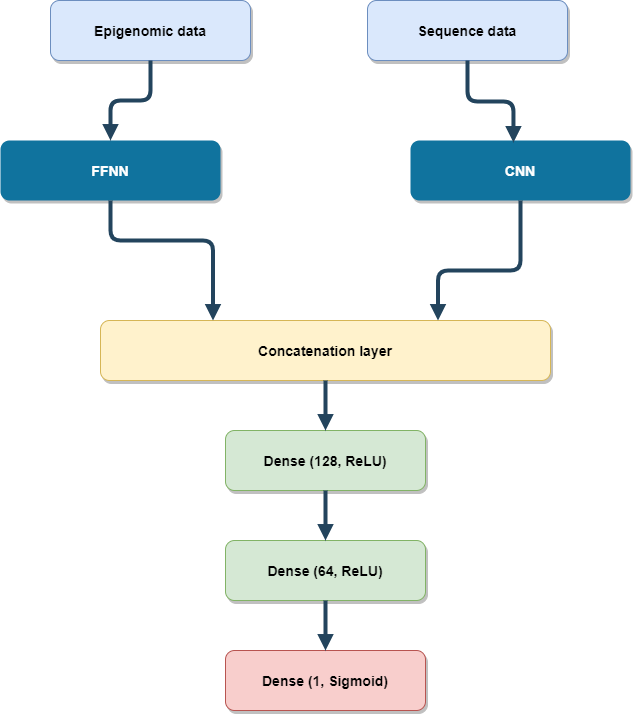
\includegraphics[width=\textwidth]{img/mmnn.png}
    \caption{MMNN architecture representation.}
    \label{fig:models:mmnn}
\end{figure}

\paragraph{MMNN.} For the MMNN we applied an intermediate integration strategy \cite{li_wu16}, in which the last hidden layers of the FFNN and the CNN are joined in a concatenation layer. This new layer is followed by a small stack of fully-connected layers with ReLU activation functions, terminating in a final neuron with a sigmoid activation function. An alternative intermediate integration strategy, having also regularization properties, is illustrated in \cite{choi19}.

We show in Figure \ref{fig:models:mmnn} the layout of the MMNN, noting that no automated hyperparameter tuning has been performed on this neural network. No additional regularization methods were used in the final part of the MMNN. 

The remaining hyperparameters, involving the optimization algorithm and the training of the neural network, were set to the same values already described for the FFNN and CNN. In particular, we used a learning rate of 0.001, which was the default in the TensorFlow implementation of Nadam.

\subsection{Hyperparameter optimization}
\label{subsec:hyperparam_opt}

Deep learning algorithms possess a large number of hyperparameters. Manually searching for the optimal combination of hyperparameter values that minimizes the generalization error can be a daunting task. For this reason, well-known model selection algorithms such as grid search or random search are often employed to automatically explore hyperparameter spaces.

To achieve good results while keeping an acceptable computational cost, new hyperparameter optimization algorithms have been recently developed. We opted to use Hyperband (2018), which treats hyperparameter optimization as an infinite-armed bandit problem \cite{li18hyperband}: having a fixed amount of resources (e.g., time) and a large number of hyperparameter configurations, we have to decide whether to allocate a small quantity of resources to train each of a large number of configurations or to allocate a large quantity of resources to train models longer, but considering fewer configurations. 

Hyperband builds upon the Successive Halving algorithm idea of iteratively allocating a fixed amount of resources to a set of configurations, evaluating the configurations and then throwing out the worst half until a single configuration remains. In practice, Hyperband works by organizing subsequent brackets. In the first bracket a large number of configurations is explored, allocating a small amount of resources to each configuration (i.e., a small number of epochs for training). The best configurations are kept through the next bracket and allowed an increased amount of resources. In the last bracket, each configuration is allocated the maximum amount of resources and the best configuration is then proposed as the solution.

According to the researchers who developed Hyperband, this novel algorithm is more robust and up to 30 times faster than Bayesian optimization (BO), though possibly achieving slightly inferior solutions than some BO variants.

Ultimately, apart from speed, what motivated our decision to adopt Hyperband was the fact that this algorithm natively supports conditional hyperparameters in the search space. Although studies are being conducted in this direction also for BO \cite{levesque17}, popular libraries have yet to include BO support for conditional hyperparameters, whereas this feature is already integrated in the Hyperband implementation for Keras and TensorFlow \cite{kerastuner}.

The ability to exploit conditional hyperparameters is crucial to save time when, for instance, the second level of the FFNN or CNN architecture does not have any layer in a given configuration.

\subsection{Comparison models}
\label{subsec:comparison_models}

The models briefly listed below have been used as comparison models to gauge the performances of the FFNN, CNN and MMNN models proposed in this report. Some of these comparison models, in the papers that introduced them, were intended to be used with input of different shape, or with different data, or for different tasks than those considered here. As such, these comparison models should be regarded more as reference architectures rather than actual published models. This should be kept in mind when comparing and contrasting the results obtained from these models.

When available, these comparison models were adapted from the code sources provided by the respective Authors, using the hyperparameter values either mentioned in the papers or set in the corresponding implementation.

\paragraph{DeepEnhancer.} This is a CNN described in \cite{min17} with the purpose of distinguishing enhancers from background genomic sequences, using only one-hot encoded sequence data. The best variation of this CNN, labeled  “4conv2pool4norm" by the Authors, consists of 4 convolutional layers followed by batch normalization, with a max pooling layer every two consecutive convolutional layers. The network ends with two fully-connected layers interleaved with a dropout layer and a single neuron with a sigmoid activation function on top.

\paragraph{Bayesian-FFNN and Bayesian-CNN.} These networks were proposed in \cite{cappelletti20} for the same tasks we are considering in this report, although human genome  “HG19" instead of  “HG38" was used. Nonetheless, the FFNN was trained on epigenomic data, while the CNN was trained on sequence data.

The Bayesian-FFNN consists of 3 fully-connected layers, with a ReLU activation function, stacked on top of each other and terminating in a single neuron with a sigmoid activation function. Additionally, $L^2$ parameter regularization is enforced for each hidden layer. To minimize the loss function, the Authors employed Stochastic Gradient Descent (SGD) with a learning rate decay schedule.

The Bayesian-CNN consists of 4 convolutional layers followed by batch normalization, with a max pooling layer after the third and fourth layers. Then 2 fully-connected layers followed by dropout layers are added, with a final neuron having a sigmoid activation function. Here the Nadam algorithm is used for optimization.

\paragraph{DeepCAPE.} DeepCAPE is a complex network described in \cite{chen21} with the purpose of predicting enhancers. The network incorporates two different CNNs trained on sequence data and on DNase-seq data. Owing to the small number of replicates in DNase-seq data and differences between cell lines, an autoencoder antecedes the CNN dealing with this kind of data. Both CNNs are then joined in a concatenation layer, culminating in a stack of 3 fully-connected layers with a dropout layer. The Authors mentioned using the Adam \cite{kingma15} optimizer.

The peculiarity of this network is represented by its intensive use of shortcut (or skip) connections reminiscent of those employed in the renowned ResNet neural network for image classification \cite{he15resnet}. With these connections, many of the intermediate layers from both CNNs are directly tied to the concatenation layer. Such connections, among other properties, counteract the vanishing gradient problem, allowing for deeper networks that can be trained faster.

For the sake of making a fair comparison with other architectures without feeding different kinds of data to the models, in our experiments we used only the CNN trained on sequence data, while keeping the final fully-connected layers and the corresponding connections when possible.

\paragraph{DECODE.} DECODE is a CNN illustrated in \cite{chen_zhang21} aimed at predicting enhancers. However, this CNN is not trained on sequence data, but on epigenetic features extracted from STARR-seq, DNase-seq, ATAC-seq and ChIP-seq data.

The architecture displays 4 convolutional layers followed by a max pooling layer, then other 3 convolutional layers followed by another max pooling layer, and finally a fully-connected layer followed by a single neuron with sigmoid activation function. Optimization is carried out by the Adam algorithm with a learning rate of 5e-5.

Another characteristic of DECODE is that each convolutional layer is endowed with a sqeeze-and-excitation block, consisting of a global average pooling layer and two fully-connected layers acting as a gate which determines how many of the features are kept.

\paragraph{Random Forest.} To gain insights into the performance of alternative machine learning algorithms, we also employed Random Forest \cite{leo01rf} as a comparison model. The implementation of this algorithm was taken from \texttt{scikit-learn} (hereinafter also \texttt{sklearn}) \cite{scikit-learn}. Random Forest was trained only on epigenomic data.

\section{Experimental setup}
\label{sec:experimental_setup}

In this section we will provide the relevant specifics of the machine used in the experiments (Subsection \ref{subsec:exp:machine}), we will explain in greater detail what the carried out tasks entail (Subsection \ref{subsec:exp:task}), the type of data and their sources (Subsection \ref{subsec:exp:data}), the data pre-processing pipeline (Subsection \ref{subsec:exp:data_preprocessing}), the ratios between samples/features and class labels (Subsection \ref{subsec:exp:ratios}), what correlations and distributions exist within the data (Subsection \ref{subsec:exp:correlations}), what feature selection algorithm was adopted (Subsection \ref{subsec:exp:feature_sel}), how the data can be visualized (Subsection \ref{subsec:exp:visualization}), how the holdouts have been planned (Subsection \ref{subsec:exp:holdouts}), what metrics have been used to evaluate the models (Subsection \ref{subsec:exp:metrics}).


\subsection{Machine specifics}
\label{subsec:exp:machine}

The experiments were run on a machine with an Intel(R) Core(TM) i7-9700K 3.60GHz 8 core processor and 16 GB of RAM. To speed up the neural networks training, a NVIDIA(R) GeForce(R) RTX 2070 SUPER(TM) was employed.

The code was written in the Python language, using Python 3.9. To implement the neural networks, we used TensorFlow 2.5.0 \cite{tensorflow2015-whitepaper}.

\subsection{Tasks description}
\label{subsec:exp:task}

Starting from the epigenomic and sequence data detailed in Subsection \ref{subsec:exp:data}, we performed two tasks. The task referred to as  “AE vs IE" pursued the objective of predicting whether a regulatory region marked as  “enhancer" was associated or not with regulatory activity within a given cell line. In other terms, this was a supervised binary classification task aimed at distinguishing active enhancers from inactive enhancers in a given cell line.

The second task,  “AP vs IP", was related to an identical supervised binary classification on the same cell line, but this time the objective was to infer from the data whether a regulatory region marked as  “promoter" was active or inactive.

Ultimately, the goal of these tasks was to provide a Machine Learning (ML) method that would be able to reliably classify as active or inactive those regulatory regions for which, currently, we do not have any label.


\subsection{Data types and sources}
\label{subsec:exp:data}

The data sources and types reflect those used in \cite{cappelletti20, li_wasserman18}. The epigenomic data were downloaded from the ENCODE Consortium \cite{encode12, encode17}, with genomic assembly  “HG38", cell line  “HepG2" and a window size of 256. These data were extracted from histone modification and TF binding ChIP-seq, DNase-seq, ATAC-seq and WGBS-seq assays marked with the  “released" status on the ENCODE portal.

The window size refers to the number of base pairs considered for each regulatory region. For enhancers, the window is centered on the activation peak for the given region. For promoters, we picked the window that starts from the peak and then covers the sequence of nucleotides in the opposite direction of the gene, which may be on the left or on the right of the peak depending on the DNA strand we are considering.    

The genomic sequence data were downloaded from the UCSC Genome Browser database \cite{ucsc20}, considering again genomic assembly  “HG38". The data were then one-hot encoded.

The ground truth labels identifying each region as an active or inactive enhancer or promoter were retrieved from the FANTOM Consortium \cite{fantom15, fantom18}, considering genomic assembly  “HG38". 

In particular, the FANTOM5 project used cap analysis of gene expression (CAGE) to identify transcriptionally active regions. From CAGE, FANTOM researchers obtained real values measured in Transcripts Per Kilobase Million (TPM). Two thresholds are then set: the minimum TPM value to consider a region active and the maximum TPM value to consider a region inactive. Obviously, the minimum TPM value for active regions should be greater than the maximum TPM value for inactive regions. Values between these two thresholds are deemed as  “gray zone values" and consequently dropped.

\begin{figure}
    \centering
    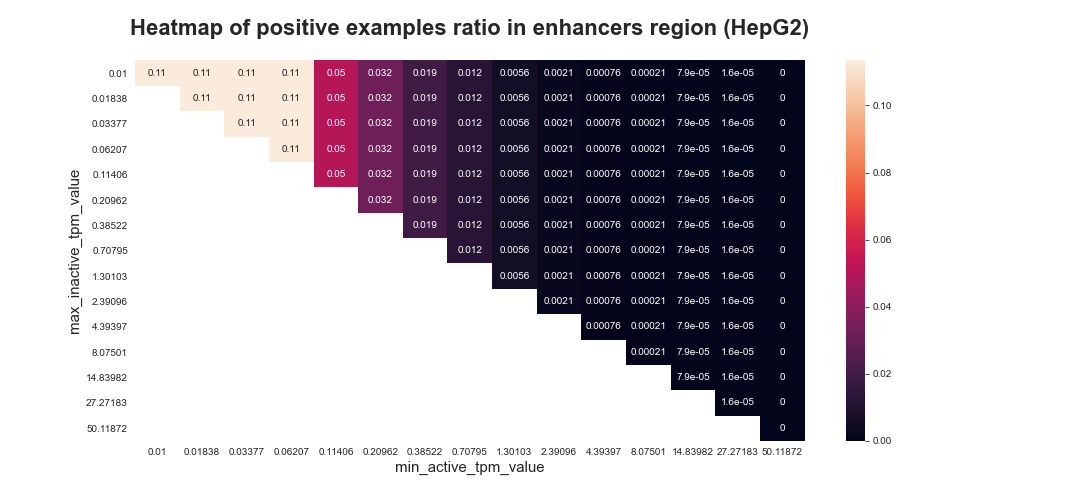
\includegraphics[width=\textwidth]{img/heatmap_HepG2_enhancers.png}
    \caption{Heatmap showing how TPM threshold values affect the positive examples ratio in the enhancers data set for cell line  “HepG2".}
    \label{fig:exp:heatmap_tpm_enh}
\end{figure}

\begin{figure}
    \centering
    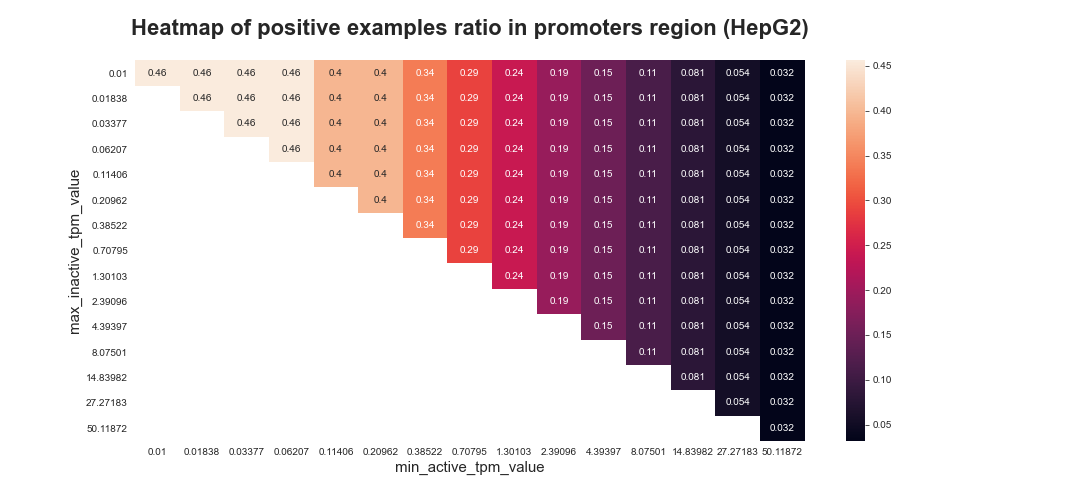
\includegraphics[width=\textwidth]{img/heatmap_HepG2_promoters.png}
    \caption{Heatmap showing how TPM threshold values affect the positive examples ratio in the promoters data set for cell line  “HepG2".}
    \label{fig:exp:heatmap_tpm_prom}
\end{figure}

Determining the optimal threshold values is an active field of research. In Figures \ref{fig:exp:heatmap_tpm_enh} and \ref{fig:exp:heatmap_tpm_prom} we produce heatmaps showing how different threshold values impact the ratio between positive and negative examples in the enhancers and promoters data sets for cell line  “HepG2". The threshold values were sampled from a log scale evenly spaced interval of 15 values, with a minimum value of $10^{-2}$ and a maximum value of $10^{1.7}$.

\begin{figure}
    \centering
    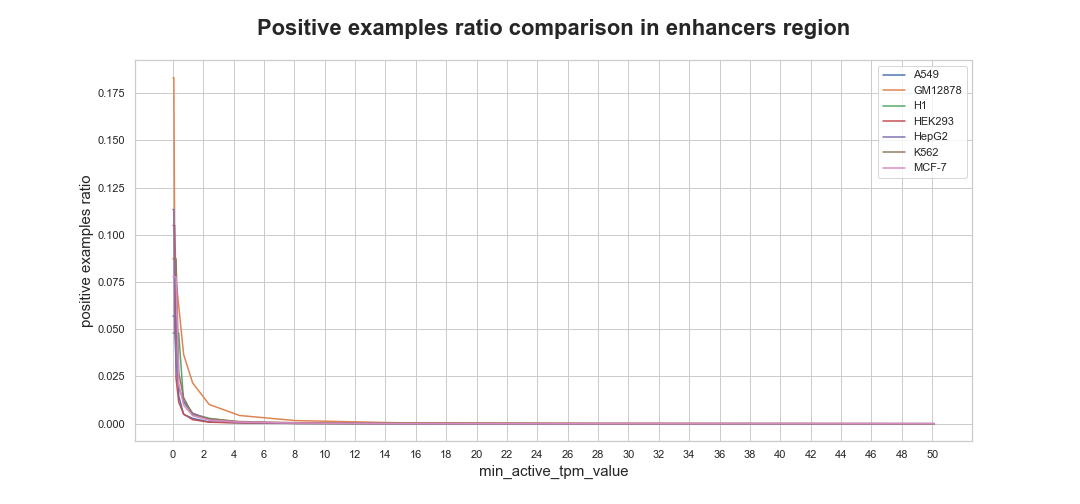
\includegraphics[width=\textwidth]{img/lineplot_enhancers.png}
    \caption{Line plot showing how the minimum TPM value to consider an enhancer region as active affects the positive examples ratio across all the available cell lines.}
    \label{fig:exp:lineplot_enh}
\end{figure}

\begin{figure}
    \centering
    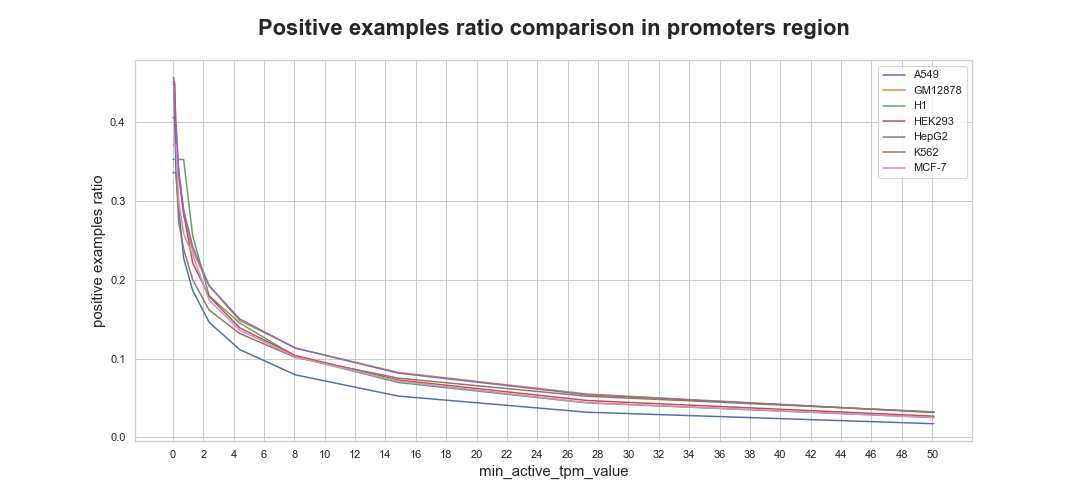
\includegraphics[width=\textwidth]{img/lineplot_promoters.png}
    \caption{Line plot showing how the minimum TPM value to consider a promoter region as active affects the positive examples ratio across all the available cell lines.}
    \label{fig:exp:lineplot_prom}
\end{figure}

In Figures \ref{fig:exp:lineplot_enh} and \ref{fig:exp:lineplot_prom} we can glimpse at the behavior of the positive examples ratio across all the available cell lines, depending on the minimum TPM value to consider a region as active. Clearly, for all the cell lines the ratio decreases monotonically as the threshold increases. Since the function is monotonic, no hints are given as to what the optimal threshold value could be. In other contexts, such as metrics used to evaluate unsupervised clustering based on monotonic functions, like the RMSSTD, R-Squared and Modified Huber $\Gamma$ metrics, it is considered optimal the point where the bend of the curve is most steep, which is referred to as  “knee" or  “elbow" in literature \cite{halkidi01, liu13}. Here we note that such elbow appears to be located at around 0.5 and 1 for enhancers and around 5 and 7 for promoters.

In \cite{li_wasserman18}, the Authors, using genomic assembly  “HG19", chose minimum active values of 0 and 5, respectively for enhancers and promoters; and considered as inactive enhancers and promoters having a TPM equal to 0. FANTOM researchers suggest using an active threshold of 1 TPM for both enhancers and promoters, dropping values between 0 and 1. We adopted this last solution for our experiments.

Useful tools to automate the process of retrieving the data, using the Python language, are provided by the following \texttt{pip} packages: \texttt{epigenomic\_dataset}\footnote{\url{https://github.com/AnacletoLAB/epigenomic_dataset}} and \texttt{ucsc\_genomes\_downloader}\footnote{\url{https://github.com/LucaCappelletti94/ucsc_genomes_downloader}}.


\subsection{Data pre-processing}
\label{subsec:exp:data_preprocessing}

The epigenomic data for the enhancers contained 19 NaN values out of 35566170 total values, while the epigenomic data for the promoters contained 359 NaN values out of 56133122 total values. In both cases, the WGSB-seq assay accounted for most of the NaN values.

Given the limited amount of NaN values, imputation of the missing values in the epigenomic data was feasible. To accomplish this task, we opted for the \texttt{KNNImputer} class made available by \texttt{sklearn}. It is worth to note that the \texttt{KNNImputer} was fitted using only the training set to avoid any possible data leakage. The fitted imputer was then applied to transform the training, validation and test sets.

Upon the epigenomic data we also performed normalization by means of the \texttt{RobustScaler} class of \texttt{sklearn}. In this way we standardized the dataset by centering the values to the median and then scaling according to the interquartile range, so that possible outliers were not taken into account during the process. Again, the scaler was fitted only on the training set.

As for the sequence data, only one nucleotide remained unidentified for enhancers, while 4 nucleotides remained unidentified for promoters. In this case, the solution was to use 0.25 as a filler value when one-hot encoding the unknown nucleotides.


\subsection{Samples/features and class labels ratios}
\label{subsec:exp:ratios}

\begin{figure}
    \centering
    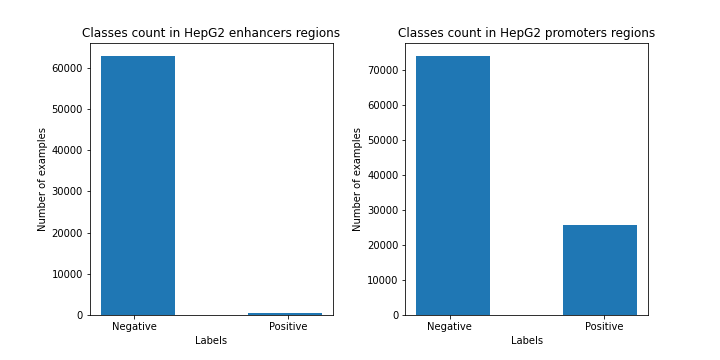
\includegraphics[width=\textwidth]{img/classes_count.png}
    \caption{Class imbalance in the enhancers and promoters data sets.}
    \label{fig:exp:class_imbalance}
\end{figure}

In this subsection we briefly comment on the ratios between features and samples and on the imbalance of the class labels.

\paragraph{Samples/features ratio.} Considering the epigenomic data, the ratio between samples and features was $\approx 112.606$ for enhancers and $\approx 177.724$ for promoters. With data having a strongly imbalanced ratio between samples and features, it is possible to find a single feature that, purely by chance, is able to correctly discriminate the classes of the data. If that was the case, the predictions made by the models would not be reliable on different data sets. In this case it is safe to assume that the ratios are within a reasonable range.

\paragraph{Class imbalance.} The classes of the data set, for both enhancers and promoters, are not balanced, as shown in Figure \ref{fig:exp:class_imbalance}. More precisely, $\approx 0.992\%$ of the enhancers are inactive, while $\approx 0.008\%$ are active; concerning the promoters, $\approx 0.742\%$ are inactive, while $\approx 0.258\%$ are active. Possible strategies to address the class imbalance issue include:
\begin{itemize}
    \item over-sampling, which balances the classes by increasing the number of instances of the under-represented class (for example, using the SMOTE algorithm \cite{chawla02smote});
    \item under-sampling, which balances the classes by decreasing the number of instances of the over-represented class;
    \item specific class weights for the neural networks, so that errors on the under-represented class have more impact on the loss function\footnote{To compute the weights, we used the formulas found at \url{https://www.tensorflow.org/tutorials/structured_data/imbalanced_data\#class_weights}}. 
\end{itemize}

We put some of these strategies into practice during the experiments (see the Results \textit{infra}, Section \ref{sec:results}).

\subsection{Data correlations and distributions}
\label{subsec:exp:correlations}

In this subsection we focus on what features are the least correlated with the output, what features are the most correlated with each other and what is the distribution of the most different features. 

\paragraph{Output correlation.} In the context of epigenomic data, we computed Pearson correlation coefficient, Spearman correlation coefficient and Maximal information coefficient to identify the features least correlated with the output. The features we found are listed below.

\begin{itemize}
    \item Enhancers: MAFG, SNRNP70, EZH2, NBN, ZNF382, CEBPZ, ARNT, ATM.
    \item Promoters: ZNF207, ZNF737.
\end{itemize}

\begin{figure}
    \centering
    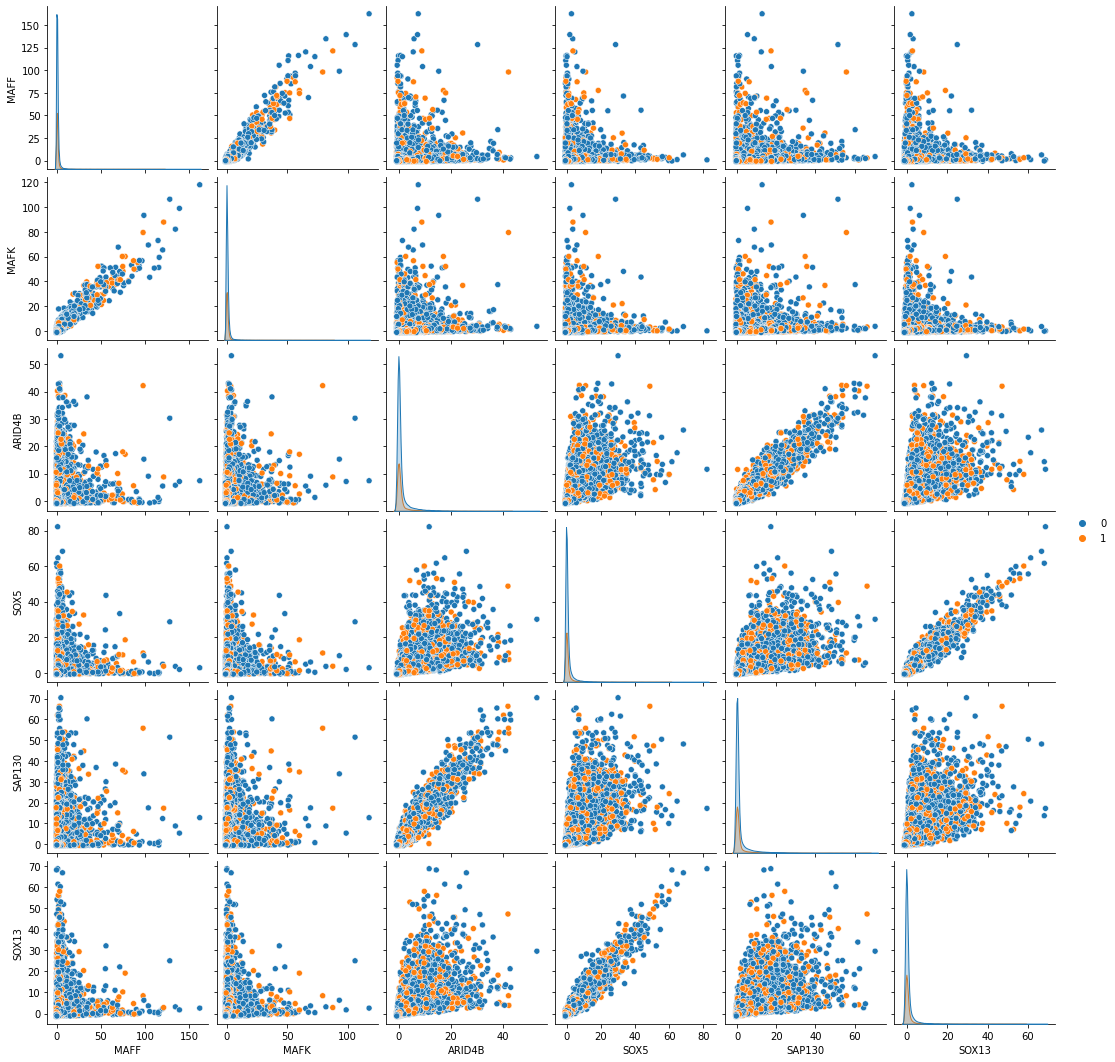
\includegraphics[width=\textwidth]{img/most_correlated_features_enhancers.png}
    \caption{Pairwise scatter plot of the most correlated features in the enhancers data set.}
    \label{fig:exp:corr_feat_enh}
\end{figure}

\begin{figure}
    \centering
    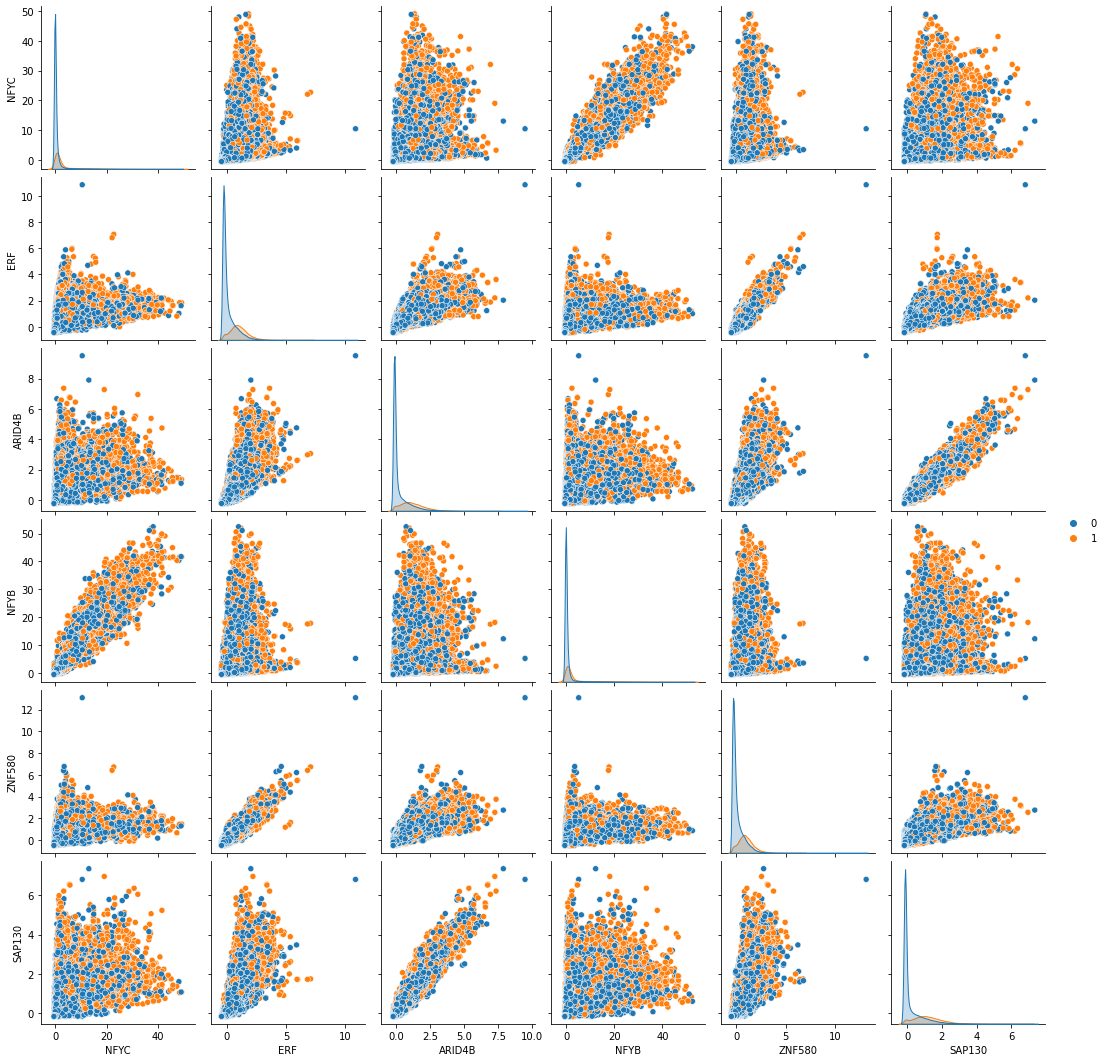
\includegraphics[width=\textwidth]{img/most_correlated_features_promoters.png}
    \caption{Pairwise scatter plot of the most correlated features in the promoters data set.}
    \label{fig:exp:corr_feat_prom}
\end{figure}

\paragraph{Feature correlation.} In Figures \ref{fig:exp:corr_feat_enh} and \ref{fig:exp:corr_feat_prom} we show the pairwise scatter plots of the features with the highest correlation. Correlation is particularly notable for SOX13-SOX5 and SAP130-ARID4B in the enhancers data set; and for ZNF580-ERF, ZBTB25-ZNF639, KLF16-ZGPAT, KLF16-ERF, ZNF274-ZNF883, SAP130-ARID4B, ZNF407-ZNF883 and NFYB-NFYC in the promoters data set.

\begin{figure}
    \centering
    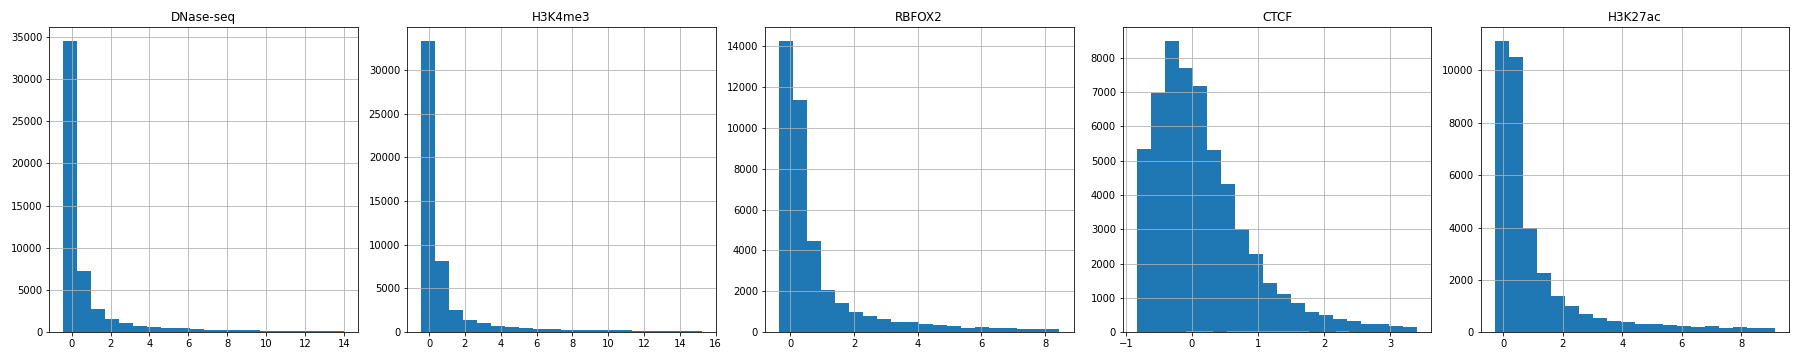
\includegraphics[width=\textwidth]{img/top_different_features_enhancers.png}
    \caption{Distributions of the most different features in the enhancers data set.}
    \label{fig:exp:distr_feat_enh}
\end{figure}

\begin{figure}
    \centering
    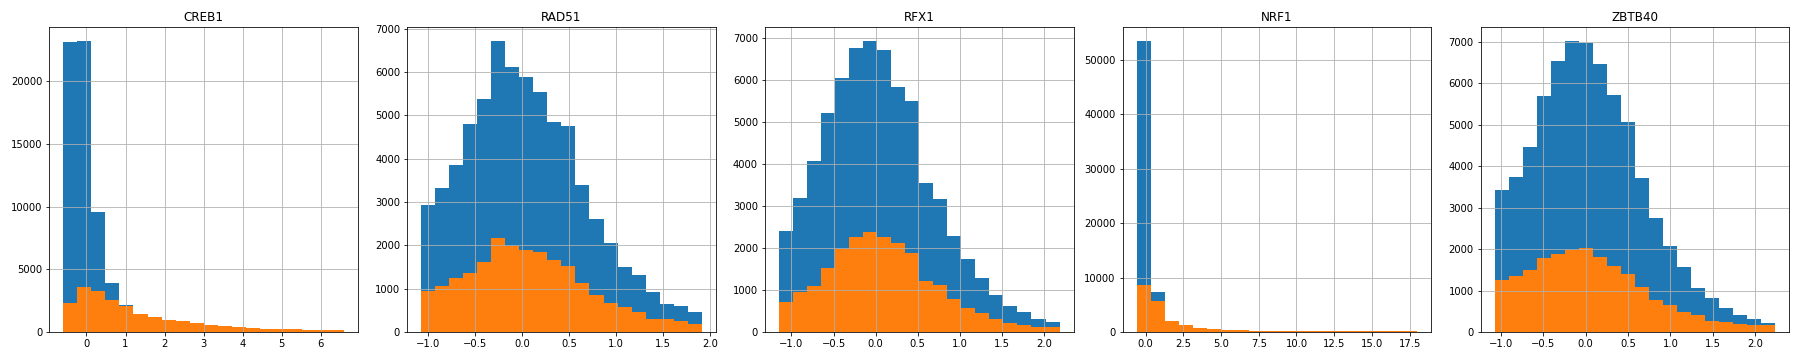
\includegraphics[width=\textwidth]{img/top_different_features_promoters.png}
    \caption{Distributions of the most different features in the promoters data set.}
    \label{fig:exp:distr_feat_prom}
\end{figure}

\paragraph{Feature distribution.} In Figures \ref{fig:exp:distr_feat_enh} and \ref{fig:exp:distr_feat_prom} we show the distributions of the five most different features, where the difference was measured by the Euclidean distance between each feature vector.

From the figures we can argue that the task of classifying active and inactive enhancers/promoters cannot be tackled with a simple linear classifier, seeing that, especially for promoters, both labels assume a similar distribution, thus making separation more difficult. Generally the distributions of the two labels are both right-skewed and either Gaussian or exponential. In the case of the promoters, we also have a spike located mainly in the same position for the two labels. In the enhancers data set, the small number of positive examples makes it difficult to attain useful insights on the distributions of the labels.

\subsection{Feature selection}
\label{subsec:exp:feature_sel}

The epigenomic data are composed of 562 features. To reduce the number of features, keeping only the most relevant ones and removing any possible noise, we performed feature selection by means of the Boruta algorithm \cite{kursa10boruta}. We availed ourselves of the Python implementation offered by the \texttt{BorutaPy} package\footnote{\url{https://github.com/scikit-learn-contrib/boruta_py}}.

Boruta wraps a Random Forest classifier, which provides a ranking of the importance of the features with respect to the loss of the accuracy of classification. Boruta then adds to the data set  “shadow" features obtained by shuffling the values of the original features. The importance of these shadow features is used to determine which features are truly relevant.

Concerning Boruta's hyperparameters, we built a Random Forest classifier from \texttt{sklearn} with a maximum depth of 5 and a balanced subsample class weight. Boruta was run for 100 iterations with the alpha hyperparameter set to 0.05 and the number of estimators set to  “auto".

Like we did for imputation and normalization, Boruta was fitted only on the training set.

\subsection{Data visualization}
\label{subsec:exp:visualization}

\begin{figure}
    \centering
    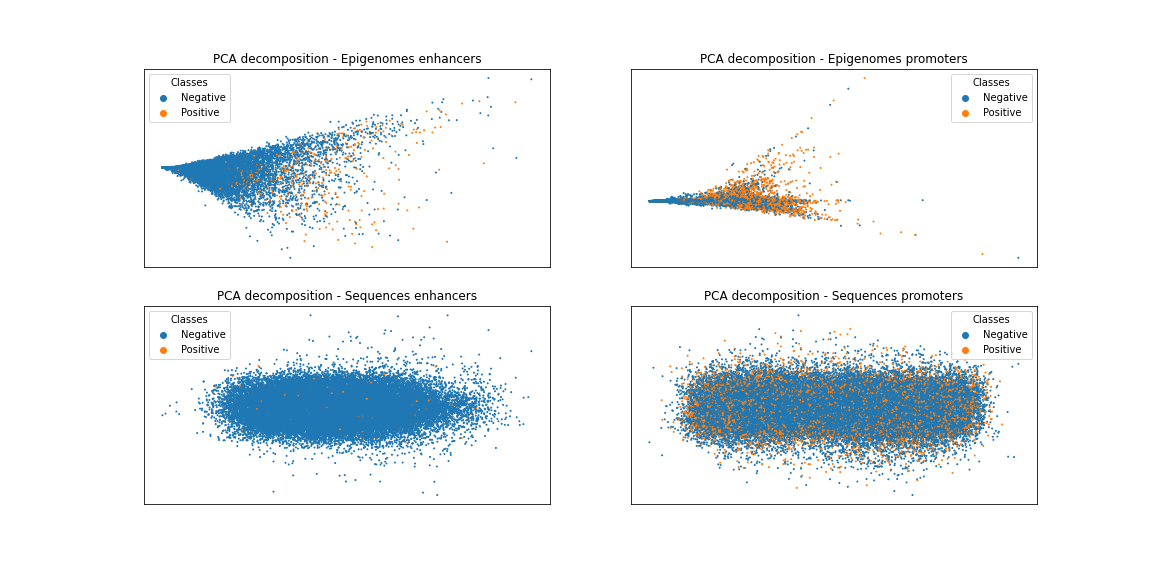
\includegraphics[width=\textwidth]{img/pca.png}
    \caption{Data visualization using PCA for dimensionality reduction.}
    \label{fig:exp:data_viz_pca}
\end{figure}

\begin{figure}
    \centering
    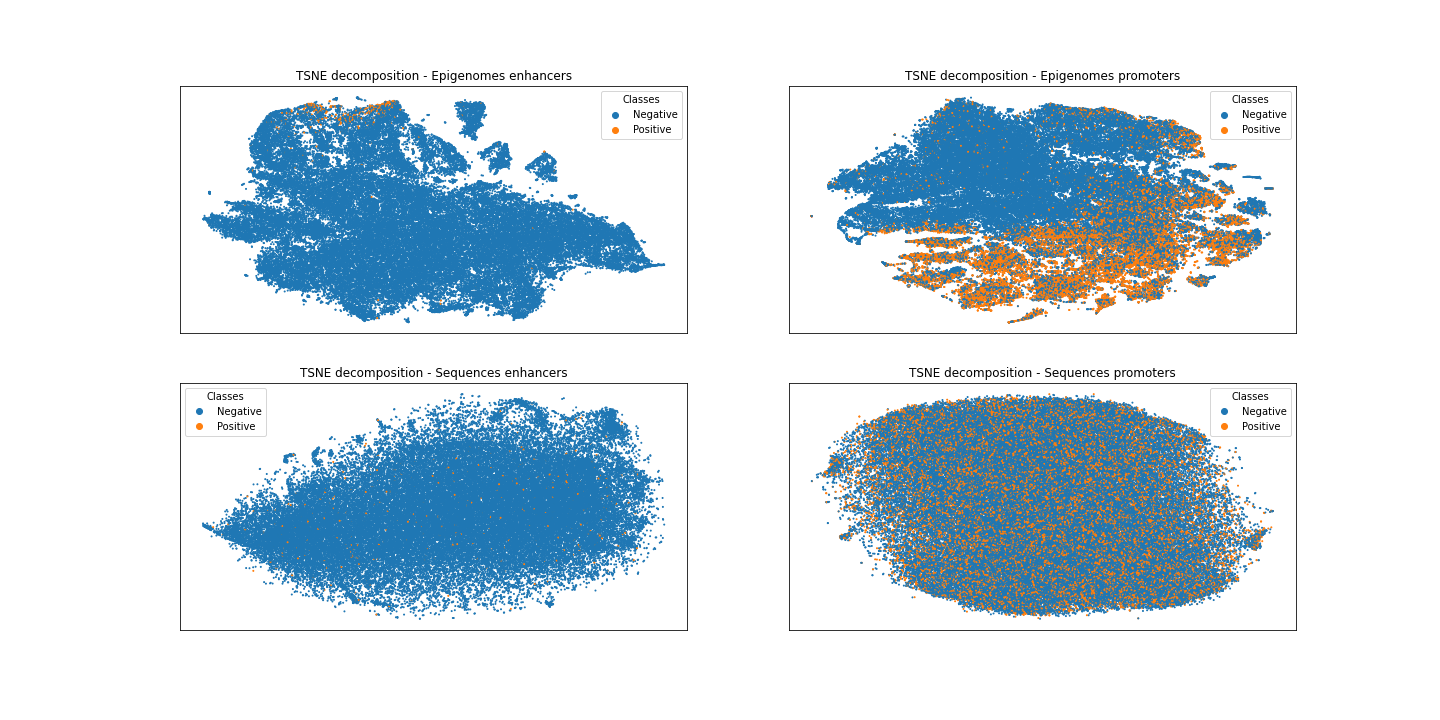
\includegraphics[width=\textwidth]{img/50_tsne.png}
    \caption{Data visualization using t-SNE for dimensionality reduction, with perplexity set to 50.}
    \label{fig:exp:data_viz_tsne}
\end{figure}

Figures \ref{fig:exp:data_viz_pca} and \ref{fig:exp:data_viz_tsne} respectively visualize data by applying two well-known dimensionality reduction algorithms: Principal Component Analysis (PCA), in the implementation provided by \texttt{sklearn}; and t-distributed Stochastic Neighbor Embedding (t-SNE), in the implementation provided by the \texttt{MulticoreTSNE} package\footnote{\url{https://github.com/DmitryUlyanov/Multicore-TSNE}}. Before applying the algorithms, we performed imputation and normalization on the whole data sets. A form of data scaling is especially useful to obtain a meaningful representation from PCA.

Both the PCA and t-SNE plots support the conclusion that, while the epigenomic data sets offer some degree of separation between the two classes, the sequence data sets make hardly any distinction possible. This consolidates the claim that classification based on sequence data is a more difficult task. However, it should be kept in mind that this conclusion is drawn from two-dimensional data, which may or may not serve as a reliable indication of the separability of the two classes in the original high-dimensional space.    


\subsection{Holdouts}
\label{subsec:exp:holdouts}

In order to evaluate the models we executed 10 holdouts, each of which, after shuffling the data, split the data sets in a training set containing 80\% of the data and in a test set containing the remaining 20\% of the data. In doing so, we preserved the stratification of the classes in both the training and test sets.

Within each holdout, we also extracted a validation set from the training set, following the same procedure described above. So we ended up with a training set containing 80\% of the data of the original training set and a validation set containing the remaining 20\% of the data of the original training set. The validation set was then employed during the model selection for the FFNN and CNN meta-models and during the training of the neural networks, playing an important role within the early stopping algorithm.

The importance of having a validation set could not be overstated. While having a validation set for model selection is required to avoid an overly optimistic evaluation of the chosen model, it should be stressed that a validation set should be employed also during the training of the chosen model, when the early stopping algorithm is in place. Indeed, early stopping is part of the learning machine and should not have access to the test set before the final evaluation, if we want to keep our models from becoming biased.

Inside the holdout loops, we performed imputation, normalization and feature selection on the epigenomic data. We reiterate that in all three occasions the algorithms were fitted using only the training sets.

For the FFNN and CNN proposed meta-models, a round of hyperparameter optimization by means of Hyperband was performed for each holdout, limiting the total number of epochs to 200 and the maximum number of epochs for each configuration to 15. We pursued maximization of the area under the precision recall curve (AUPRC) on the validation set to select the best configuration. To curb the computation time required by the hyperparameter optimization, the same optimized model obtained from the data resulting from feature selection was used with the data of the corresponding holdout for which no feature selection was performed. For each meta-model, in each holdout, the model selection phase took from 30 to 45 minutes.  

Finally, it is worth mentioning that, to feed the batches to the networks and to lazily compute the one-hot encoding of the sequence data in a memory-efficient way, we relied upon the following packages: \texttt{keras\_bed\_sequence}\footnote{\url{https://github.com/LucaCappelletti94/keras_bed_sequence}} and \texttt{keras\_mixed\-\_sequence}\footnote{\url{https://github.com/LucaCappelletti94/keras_mixed_sequence}}.


\subsection{Metrics}
\label{subsec:exp:metrics}

Each model was evaluated according to mainly three metrics: area under the precision recall curve (AUPRC), area under the receiver operating characteristic curve (AUROC) and accuracy. Given the imbalance of the classes, the mean AUPRC over the test sets was considered the most informative predictor of the quality of the model.

To gauge the existence of a statistical difference between models under comparison, we used the Wilcoxon signed-rank test. We considered a p-value lower than 0.01 as a sensible threshold to claim that the compared models were statistically different.  

\section{Results}
\label{sec:results}

\begin{figure}
    \centering
    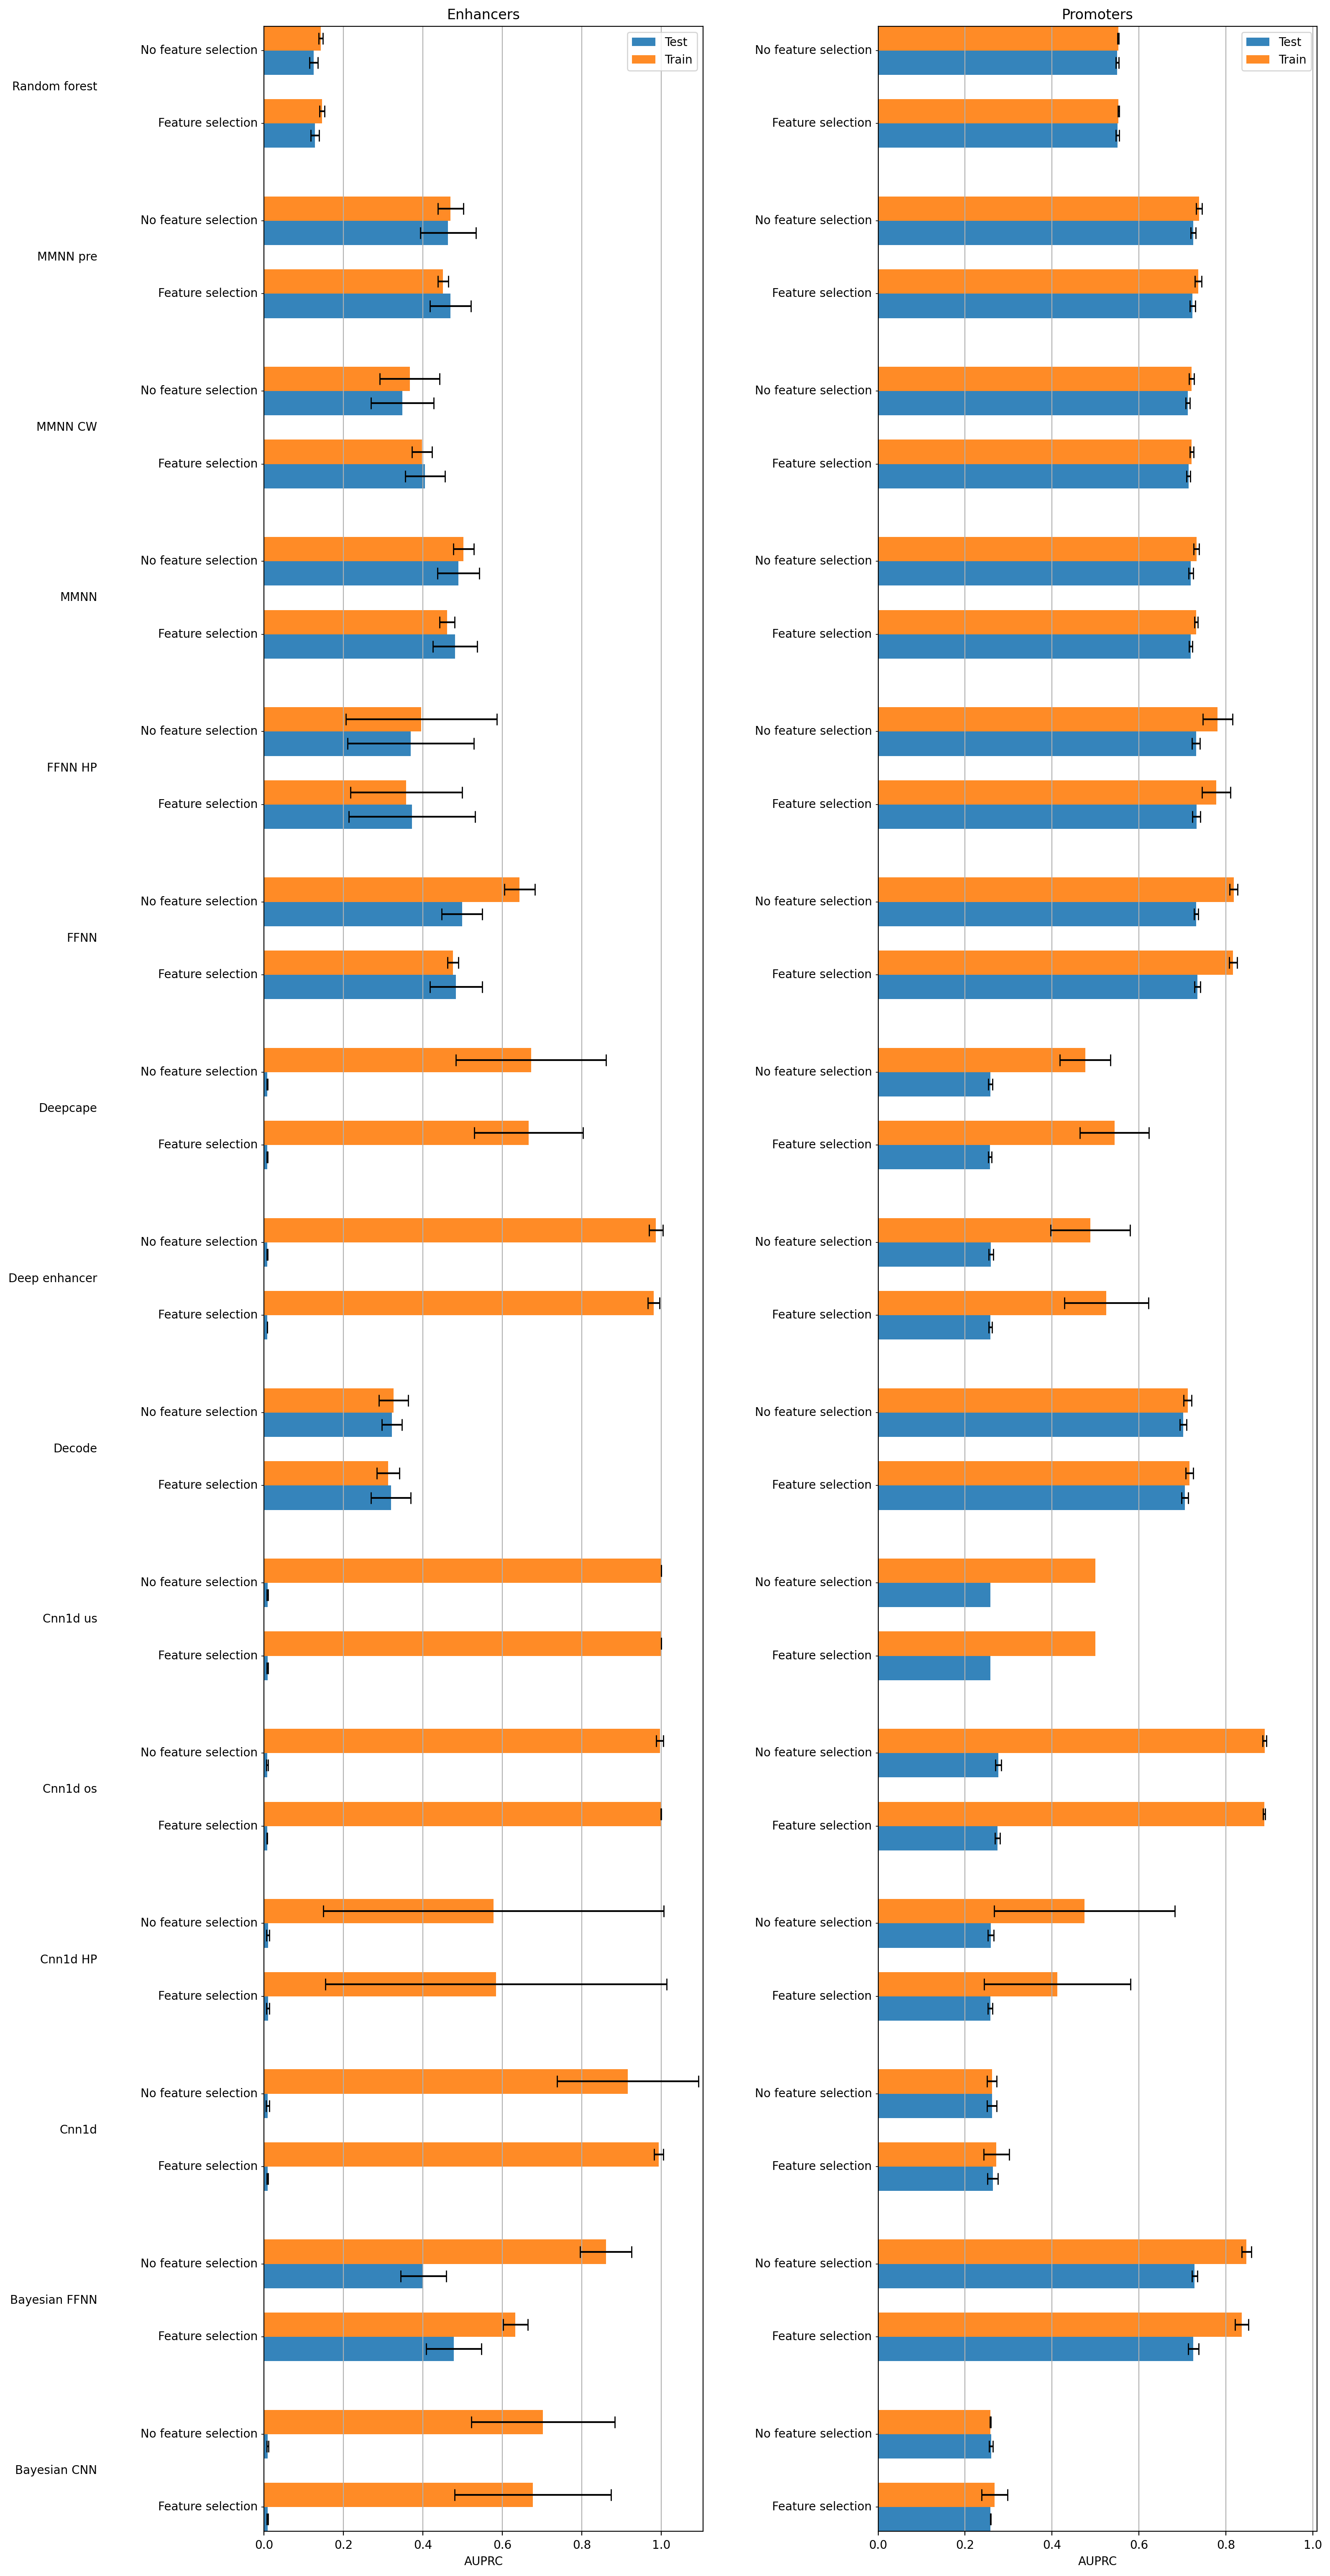
\includegraphics[height=\textheight]{img/auprc.png}
    \caption{Results of the models with the AUPRC metric.}
    \label{fig:res:auprc}
\end{figure}

\begin{figure}
    \centering
    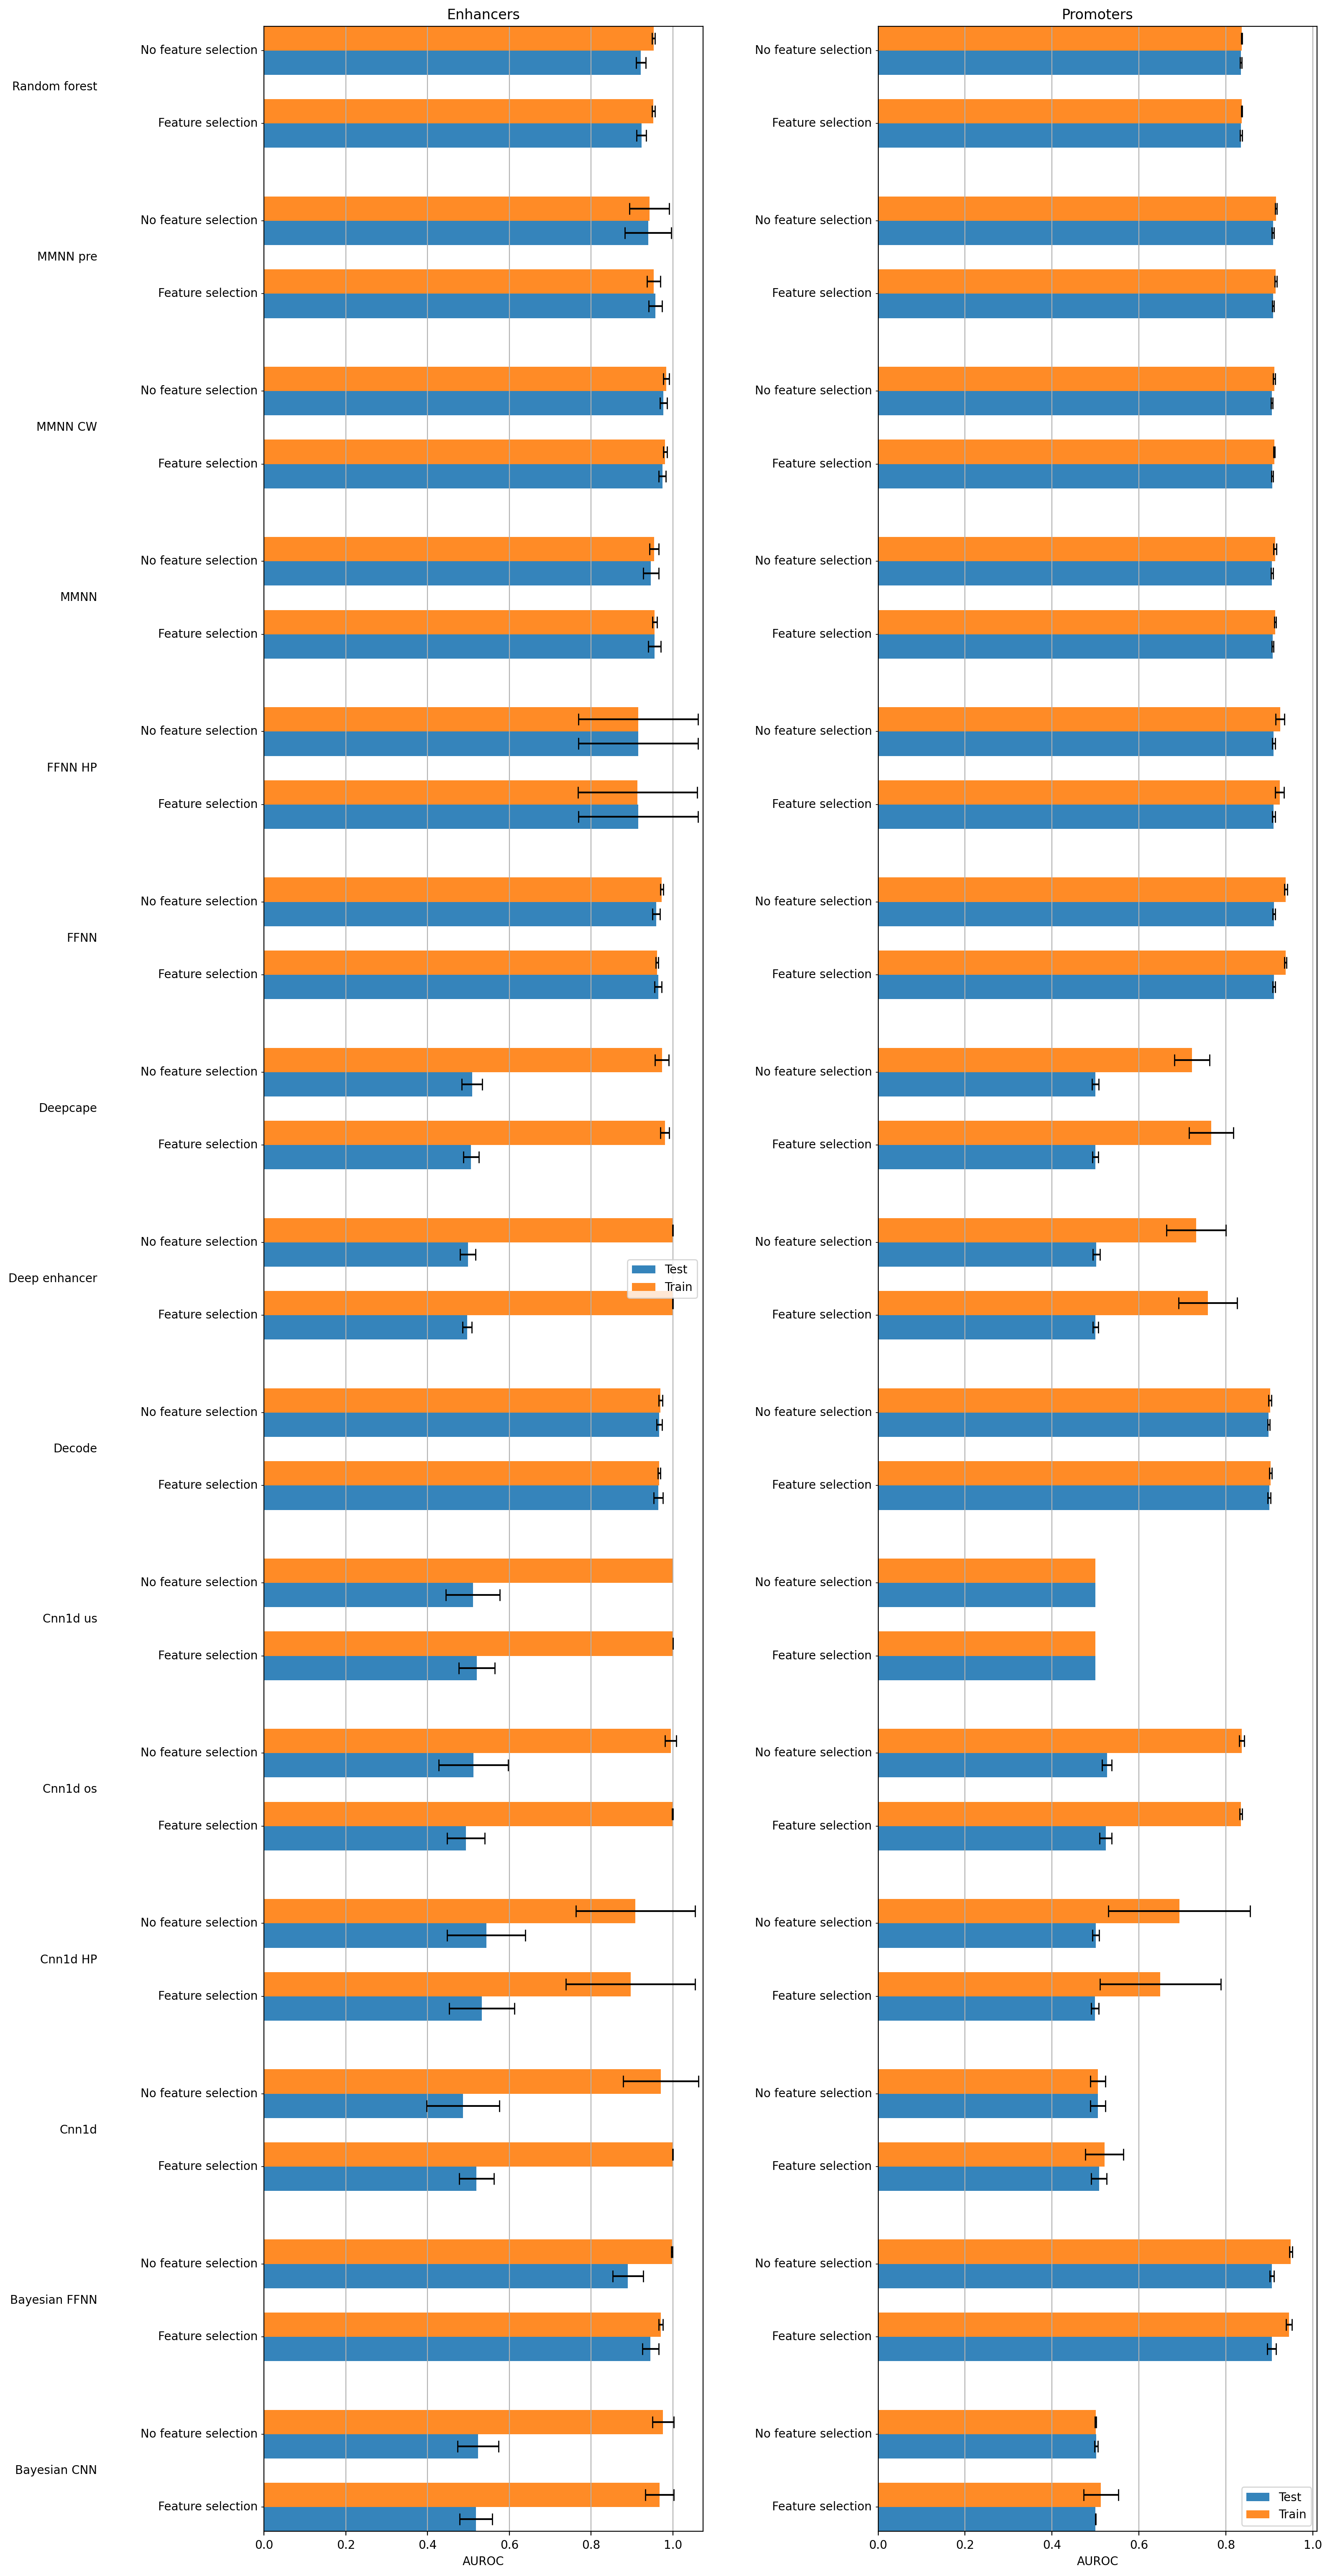
\includegraphics[height=\textheight]{img/auroc.png}
    \caption{Results of the models with the AUROC metric.}
    \label{fig:res:auroc}
\end{figure}

\begin{figure}
    \centering
    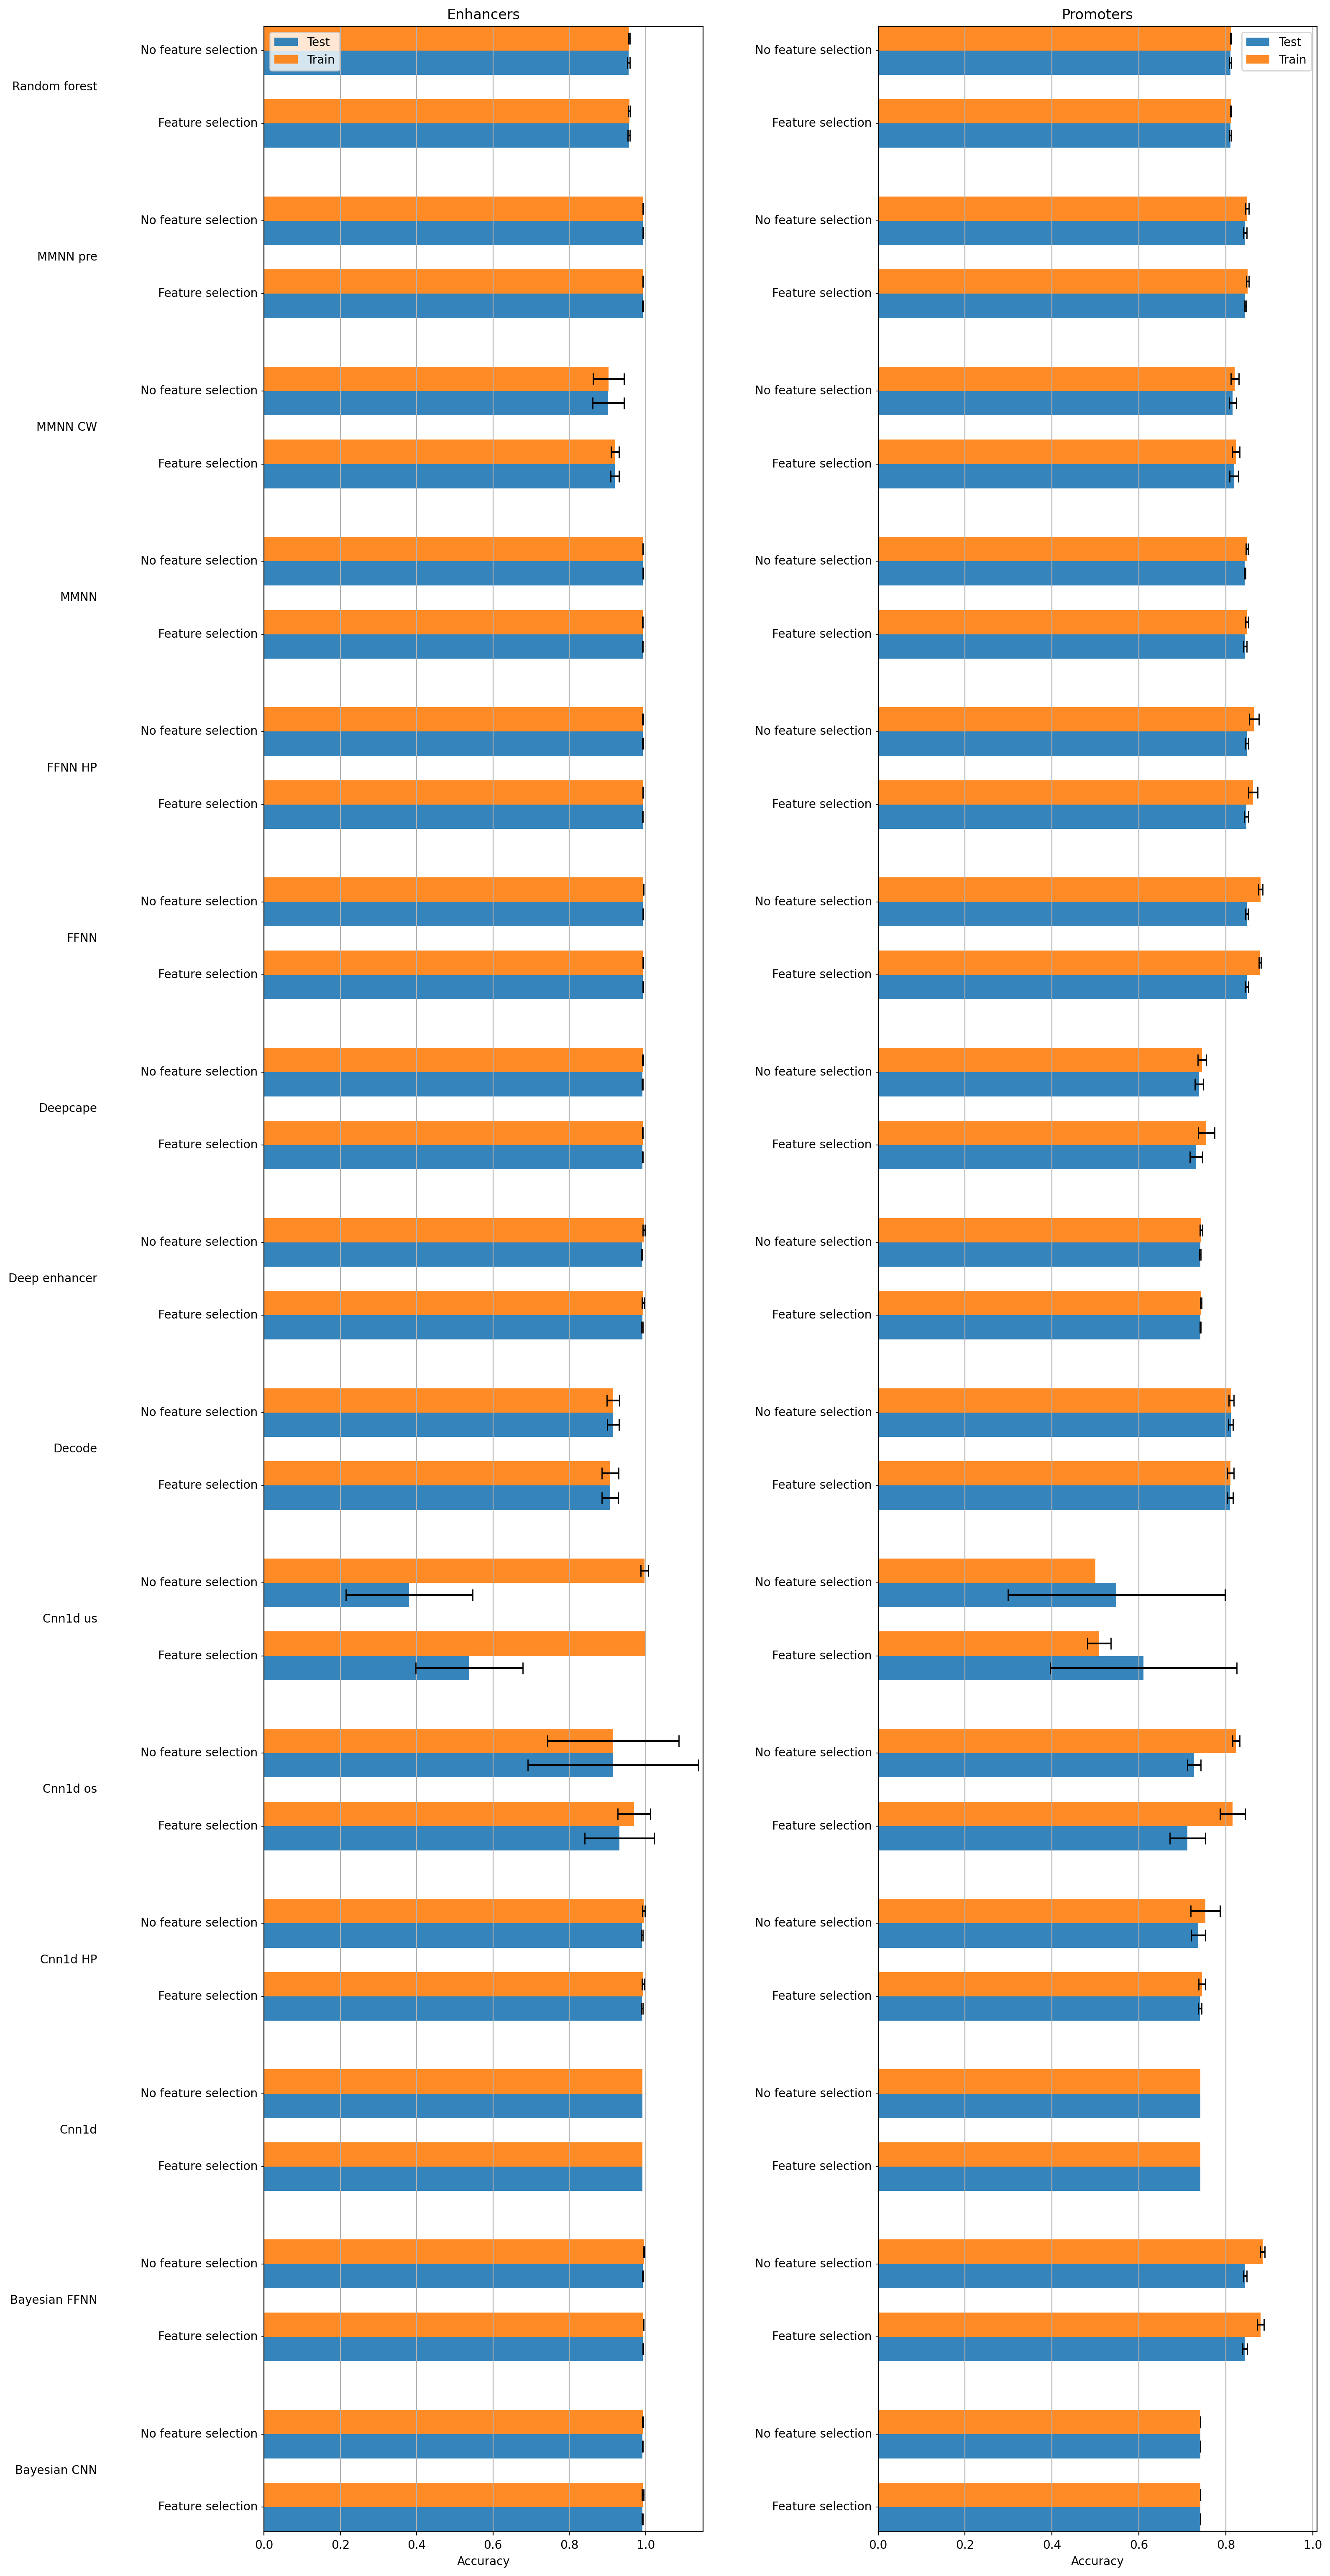
\includegraphics[height=\textheight]{img/accuracy.png}
    \caption{Results of the models with the accuracy metric.}
    \label{fig:res:accuracy}
\end{figure}

\paragraph{Naming conventions.} In the figures presented in this section, the evaluated models are referred to with the following naming conventions:

\begin{itemize}
    \item FFNN: the manually chosen feed-forward neural network;
    \item FFNN HP: the feed-forward neural network resulting from model selection on the FFNN meta-model;
    \item Cnn1d: the manually chosen convolutional neural network;
    \item Cnn1d us: the manually chosen convolutional neural network, with random under-sampling applied to the training set;
    \item Cnn1d os: the manually chosen convolutional neural network, with SMOTE over-sampling applied to the training set;
    \item Cnn1d HP: the convolutional neural network resulting from model selection on the CNN meta-model;
    \item MMNN: the multi-modal neural network trained from scratch;
    \item MMNN pre: the multi-modal neural network trained using pre-trained FFNN and CNN (FFNN and CNN layers were not frozen);
    \item MMNN cw: the multi-modal neural network trained from scratch, but with class weights applied to the loss function, to give more emphasis to the minority class.
\end{itemize}

In Figures \ref{fig:res:auprc}, \ref{fig:res:auroc} and \ref{fig:res:accuracy} we show the results obtained respectively with the AUPRC, AUROC and accuracy metrics.  

\paragraph{Feature selection relevance.} Feature selection with Boruta marked a statistically significant difference in the model performances only with the Bayesian FFNN model, over the enhancers task (p-value 0.003 for AUPRC and AUROC). Therefore, we can claim that the feature selection relevance, using Boruta, was overall negligible. In the next paragraphs, for the sake of simplicity, we will consider only the results obtained with feature selection.

\paragraph{Enhancers.} Distinguishing active and inactive enhancers was the most difficult task. Due to the class imbalance, we can consider the AUPRC scores as the most informative scores. It is evident from the figures that models trained on epigenomic data obtained the best results. In particular, FFNN, MMNN, MMNN pre and Bayesian FFNN obtained the best results, with a mean AUPRC around 0.48, and were statistically indistinguishable.

\begin{table}
    \centering
    \resizebox{\textwidth}{!}{
    \begin{tabular}{llrrrrrrrrr}
    \toprule
         region &     model\_name & \multicolumn{2}{c}{tp/t} & \multicolumn{2}{c}{fp/t} & \multicolumn{2}{c}{tn/t} & \multicolumn{2}{c}{fn/t} \\
          & & mean &       std &      mean &       std &      mean &       std &      mean &       std \\
    \midrule
      enhancers &   bayesian\_cnn &  0.000008 &  0.000025 &  0.000482 &  0.001524 &  0.991538 &  0.001524 &  0.007972 &  0.000025 \\
      enhancers &          cnn1d &  0.000000 &  0.000000 &  0.000000 &  0.000000 &  0.992020 &  0.000000 &  0.007980 &  0.000000 \\
      enhancers &       cnn1d\_hp &  0.000000 &  0.000000 &  0.001256 &  0.002040 &  0.990764 &  0.002040 &  0.007980 &  0.000000 \\
      enhancers &       cnn1d\_os &  0.000395 &  0.000592 &  0.061263 &  0.091349 &  0.930758 &  0.091349 &  0.007585 &  0.000592 \\
      enhancers &       cnn1d\_us &  0.003919 &  0.001050 &  0.458181 &  0.141164 &  0.533839 &  0.141164 &  0.004061 &  0.001050 \\
      enhancers &  deep\_enhancer &  0.000000 &  0.000000 &  0.000980 &  0.001833 &  0.991041 &  0.001833 &  0.007980 &  0.000000 \\
      enhancers &       deepcape &  0.000000 &  0.000000 &  0.000166 &  0.000405 &  0.991854 &  0.000405 &  0.007980 &  0.000000 \\
      promoters &   bayesian\_cnn &  0.000005 &  0.000016 &  0.000000 &  0.000000 &  0.741853 &  0.000000 &  0.258142 &  0.000016 \\
      promoters &          cnn1d &  0.000000 &  0.000000 &  0.000000 &  0.000000 &  0.741853 &  0.000000 &  0.258147 &  0.000000 \\
      promoters &       cnn1d\_hp &  0.000636 &  0.001517 &  0.002017 &  0.005029 &  0.739836 &  0.005029 &  0.257511 &  0.001517 \\
      promoters &       cnn1d\_os &  0.019748 &  0.024212 &  0.049582 &  0.064890 &  0.692271 &  0.064890 &  0.238399 &  0.024212 \\
      promoters &       cnn1d\_us &  0.069019 &  0.113473 &  0.200200 &  0.328045 &  0.541653 &  0.328045 &  0.189128 &  0.113473 \\
      promoters &  deep\_enhancer &  0.000240 &  0.000377 &  0.000726 &  0.000935 &  0.741127 &  0.000935 &  0.257907 &  0.000377 \\
      promoters &       deepcape &  0.005241 &  0.007660 &  0.015398 &  0.021746 &  0.726455 &  0.021746 &  0.252906 &  0.007660 \\
    \bottomrule
    \end{tabular}
    }
    \caption{True positive, false positive, true negative and false negative ratios of the test set predictions made by models trained only on sequence data with feature selection.}
    \label{tab:res:tp_tn_sequence}
\end{table}

The models trained on sequence data learned next to nothing, as it is evident from the AUPRC scores. This claim is confirmed by the AUROC scores, which are invariably set around 0.5, signifying performances comparable with that of a random classifier. Indeed, these models, which were affected by overfitting despite the regularization tools employed, in most cases achieved no true positive prediction on the test set over the 10 holdouts, as shown in Table \ref{tab:res:tp_tn_sequence}. Only the CNNs aided by over-sampling and under-sampling managed to recognize some positive examples, but at the price of many positive misclassifications, evinced by the ratio of false positive examples.

\paragraph{Promoters.} For the active promoters vs inactive promoters task, the best models were FFNN and FFNN HP, whose mean AUPRC reached a value around 0.73. These two models were statistically indistinguishable on mean AUPRC.

Again, models trained on epigenomic data performed better than models trained only on sequence data. Models trained on sequence data also showed poor learning, as seen from the true positive ratios in Table \ref{tab:res:tp_tn_sequence}, albeit some models achieved slightly better results than those obtained in the enhancers task. The lack of learning is also apparent from the mean AUROC scores, again around 0.5. For the models trained on sequence data, the higher AUPRC scores registered in the promoters task, with respect to the enhancers task, were mostly due to the less severe imbalance between the classes.   

\paragraph{MMNN relevance.} From the results obtained on mean AUPRC, we can say that using MMNN did not improve performance with respect to the isolated FFNN models. However, MMNN achieved better results than isolated CNN models.

Using pre-trained FFNN and CNN in MMNN pre did not modify the overall AUPRC performance with respect to the basic MMNN (p-value 0.019 for enhancers and p-value 0.013 for promoters). Surprisingly, using class weights in MMNN cw worsened the overall AUPRC performance with respect to the basic MMNN, and this difference was statistically significant (p-value 0.0019 for enhancers and p-value 0.0039 for promoters).

\paragraph{Hyperparameter optimization.} Results obtained by the Cnn1d HP meta-model suffered from high variability, as evidenced by the standard deviation in Figures \ref{fig:res:auprc} and \ref{fig:res:auroc}. Indeed, the chosen hyperparameter values differed much between the holdouts, running the gamut of the hyperparameter spaces. Increasing the amount of resources allocated for model selection and reducing the dimension of the hyperparameter spaces might help in alleviating this problem.

The FFNN HP meta-model incurred less variability, but the results were still worse or on par with that of other models, such as the manually chosen FFNN model.

\begin{table}
    \centering
    \resizebox{!}{0.4\textheight}{
    \begin{tabular}{lr}
    \toprule
    {} &  count \\
    \midrule
        HOXA3           &     10 \\
        MED1            &     10 \\
        THRA            &     10 \\
        ZGPAT           &     10 \\
        PHF8            &     10 \\
        ZNF574          &     10 \\
        TSC22D2         &     10 \\
        TFE3            &     10 \\
        NONO            &     10 \\
        IKZF5           &     10 \\
        SAP130          &     10 \\
        KDM1A           &     10 \\
        POLR2G          &     10 \\
        TFDP2           &     10 \\
        MYBL2           &     10 \\
        MAX             &     10 \\
        TBP             &     10 \\
        KMT2A           &     10 \\
        TAF1            &     10 \\
        ERF             &     10 \\
        YEATS4          &     10 \\
        ARID4B          &     10 \\
        KLF6            &     10 \\
        RBPJ            &     10 \\
        DRAP1           &     10 \\
        HDAC1           &     10 \\
        DNase-seq       &     10 \\
        ZSCAN9          &     10 \\
        THAP11          &     10 \\
        AFF4            &     10 \\
        MXD4            &     10 \\
        TFDP1           &     10 \\
        GATA4           &     10 \\
        SP5             &     10 \\
        HDAC2           &     10 \\
        H3K9ac          &     10 \\
        ZBED4           &     10 \\
        GATAD1          &     10 \\
        ARID4A          &     10 \\
        KAT7            &     10 \\
        POLR2A          &     10 \\
        ZFX             &     10 \\
        RBFOX2          &     10 \\
        ZNF580          &     10 \\
        ZNF331          &     10 \\
        IRF2            &     10 \\
        H3K27ac         &     10 \\
        PATZ1           &     10 \\
        ZBTB25          &     10 \\
        ZBTB7B          &     10 \\
        SMAD4           &     10 \\
        POLR2AphosphoS5 &     10 \\
        ASH2L           &     10 \\
        REST            &     10 \\
        LCOR            &     10 \\
        KAT8            &     10 \\
        KMT2B           &     10 \\
        DMAP1           &     10 \\
        KLF16           &     10 \\
        TFAP4           &     10 \\
        RXRB            &     10 \\
        ELF3            &      9 \\
    \bottomrule
    \end{tabular}
    }
    \caption{Number of times the features of the enhancers data set were chosen by Boruta over the 10 holdouts. Only the most selected features are shown.}
    \label{tab:res:enh_features}
\end{table}

\paragraph{Most relevant features.} During feature selection on the epigenomic data, Boruta returned for each holdout the most relevant features. Across all the holdouts, a total of 131 features, out of the original 562, were chosen at least once for the enhancers data set. The features selected most times are shown in Table \ref{tab:res:enh_features}. For the promoters dataset, a total of 508 feature, out of the original 562, were chosen at least once. The list of features for the promoters dataset is omitted for space sake.

We can conclude that, for the enhancers task, most epigenomic features are considered irrelevant by Boruta, with only a small set of features being consistently chosen by the feature selection algorithm. On the other hand, for the promoters task almost all the features are considered relevant at least once. 



\medskip

\bibliographystyle{acm}
\bibliography{bibtex_entries}

\end{document}
